%----------------------------------------------------------------------------------------
% Preambulo y Configuración
%----------------------------------------------------------------------------------------

\documentclass[
    11pt,
    spanish,
    singlespacing,
    parskip,
    headsepline,
    bookmarks=true,
    unicode=true,
    pdftoolbar=true,
    pdfmenubar=true,
    pdffitwindow=false,
    colorlinks=true,
    linkcolor=blue,
    citecolor=blue,
    urlcolor=blue
]{MastersDoctoralThesis}

% inputenc, fontenc, graphicx e hyperref ya los carga MastersDoctoralThesis.cls
\usepackage{eso-pic} % Fondos (no está en la clase)
\usepackage{float} % Colocación [H] de figuras cuando se requiere anclaje en el flujo

% Biblatex (cargado por la clase): más autores en citas narrativas y en la bibliografía; "y col." en español si aún se trunca
\ExecuteBibliographyOptions{maxcitenames=6,maxbibnames=99}
\DefineBibliographyStrings{spanish}{
  andothers = {y\space col\adddot},
  andmore = {y\space col\adddot}
}

% Opciones PDF adicionales (hyperref ya cargado por la clase)
\hypersetup{
    pdftitle={Título del Documento},
    pdfauthor={Alex D. Barria C.},
    pdfkeywords={Sistemas Embebidos, Internet de las Cosas, Inteligencia Artificial},
    pdfstartview={FitH},
    unicode=true,
    colorlinks=true,
    linkcolor=blue,
    citecolor=blue,
    urlcolor=blue
}

\pdfstringdefDisableCommands{%
  \def\texttt#1{#1}%
  \def\textbf#1{#1}%
  \def\textit#1{#1}%
  \def\"{\"}%
  \def\~{~}%
  \def\'{'}%
  \def\^{}%
  \def\textunderscore{\_} % Manejo del subrayado en marcadores
}


% Definir comandos requeridos por la clase
\newcommand{\degreename}{Maestría en Ciencias} % Cambia según tu título
\newcommand{\univname}{Universidad Nacional de Ejemplo} % Cambia según tu universidad
\newcommand{\keywordnames}{Palabras clave:}
%----------------------------------------------------------------------------------------
% Documento Principal
%----------------------------------------------------------------------------------------

\begin{document}

% Configuración de la portada
\posgrado{Carrera / Maestría}
\keywords{Sistemas Embebidos, Internet de las Cosas, Inteligencia Artificial}

% Incluir la portada desde un archivo separado
\include{portada}

% Configuración del contenido preliminar
\frontmatter % Usar numeración romana para las páginas preliminares
\pagestyle{plain} % Estilo de encabezado simple

%----------------------------------------------------------------------------------------
% Resumen
%----------------------------------------------------------------------------------------

\begin{abstract}
\addchaptertocentry{\abstractname} % Agregar resumen al índice
Este trabajo presenta el desarrollo de un sistema de software que analiza grabaciones de video de personas que realizan ejercicios estandarizados de evaluación motora en pacientes con Parkinson. La solución produce medidas cuantitativas del movimiento para complementar la valoración clínica con información objetiva y trazable. La enfermedad de Parkinson altera el control motor y suele evaluarse en consulta mediante la observación de esos ejercicios, lo que puede introducir subjetividad y dificultar el seguimiento fino de la evolución.

Para su implementación, se aplicaron contenidos de la maestría en inteligencia artificial, en particular visión por computadora, aprendizaje automático con modelos preentrenados, ingeniería de software y operaciones de aprendizaje automático.
\end{abstract}

%----------------------------------------------------------------------------------------
% Agradecimientos
%----------------------------------------------------------------------------------------

\begin{acknowledgements}
\vspace{1.5cm}
A mi familia, por el apoyo sostenido y la confianza depositada a lo largo de este recorrido formativo.

Agradezco a los docentes, autoridades y demás actores de la universidad y de la educación pública argentina que, en distintas etapas de mi formación, compartieron conocimientos, exigencia y compromiso con la enseñanza.

Reconozco también la orientación del PhD. Ing. Fernando Bernuy, director de este trabajo, y el aporte desinteresado de los distintos profesionales consultados en el ámbito clínico y técnico, cuya colaboración orientó y enriqueció aspectos centrales del presente trabajo.
\end{acknowledgements}

%----------------------------------------------------------------------------------------
% Índice
%----------------------------------------------------------------------------------------

\tableofcontents
\listoffigures
\listoftables

%----------------------------------------------------------------------------------------
% Capítulos
%----------------------------------------------------------------------------------------

\mainmatter % Iniciar numeración numérica para el contenido principal
\pagestyle{thesis} % Estilo de encabezado de tesis

% Incluir capítulos desde archivos separados
% Chapter 1

\chapter{Introducción general} % Main chapter title

\label{Chapter1} % For referencing the chapter elsewhere, use \ref{Chapter1}
\label{IntroGeneral}

En este capítulo se contextualiza la enfermedad de Parkinson, la manera habitual de evaluar sus signos motores y se expone la motivación para incorporar análisis automático de video. También se sintetiza el estado del arte en visión por computadora aplicada a trastornos del movimiento y se enuncian los objetivos del trabajo.

%----------------------------------------------------------------------------------------

\newcommand{\keyword}[1]{\textbf{#1}}
\newcommand{\tabhead}[1]{\textbf{#1}}
\newcommand{\code}[1]{\texttt{#1}}
\newcommand{\file}[1]{\texttt{\bfseries#1}}
\newcommand{\option}[1]{\texttt{\itshape#1}}
\newcommand{\grados}{$^{\circ}$}

%----------------------------------------------------------------------------------------

\section{Introducción general al tema}

La enfermedad de Parkinson es un trastorno neurodegenerativo frecuente que compromete principalmente el sistema motor. Entre sus manifestaciones se cuentan la bradicinesia, la rigidez, el temblor en reposo y alteraciones de la marcha y el equilibrio. La gravedad y la evolución de estos signos condicionan la calidad de vida del paciente y las decisiones terapéuticas del profesional de la salud.

En la práctica neurológica se emplean escalas validadas que formalizan la exploración motora. Una referencia ampliamente adoptada es la parte motora de la escala unificada de la Sociedad Internacional de Parkinson y trastornos del movimiento (MDS por su sigla en inglés), conocida en la literatura como MDS-UPDRS parte III, que guía la observación de tareas como movimientos de dedos, postura y marcha \citep{sibley2021video}. Esas puntuaciones son útiles para comparar pacientes y momentos en el tiempo, pero dependen de la pericia del examinador y del contexto de la consulta, factores que introducen variabilidad entre observadores y entre sesiones.

En los últimos años creció el interés por registrar la exploración en video, ya sea en forma presencial o remota, y por apoyar la lectura clínica con algoritmos que midan trayectorias, ritmo y amplitud a partir de las imágenes \citep{sibley2021video,pecoraro2025computer}. Esa línea de trabajo apunta a obtener descriptores cuantitativos reproducibles a partir de grabaciones convencionales, sin reemplazar al médico pero ofreciéndole un respaldo objetivo para el seguimiento.

Para situar visualmente el tipo de tareas que los profesionales solicitan durante la exploración motora, se presentan a continuación ejemplos de 4 ejercicios frecuentemente incluidos en protocolos como la parte motora de la escala MDS-UPDRS. 

En la figura \ref{fig:concepto-finger-tapping} se muestra un ejemplo de finger tapping: toques rítmicos entre el pulgar y el índice. En la imagen se observa la mano en la postura típica de la prueba, que permite al examinador valorar la amplitud, la regularidad y la fatiga del movimiento.

\vspace{0.6em}
\begin{center}
	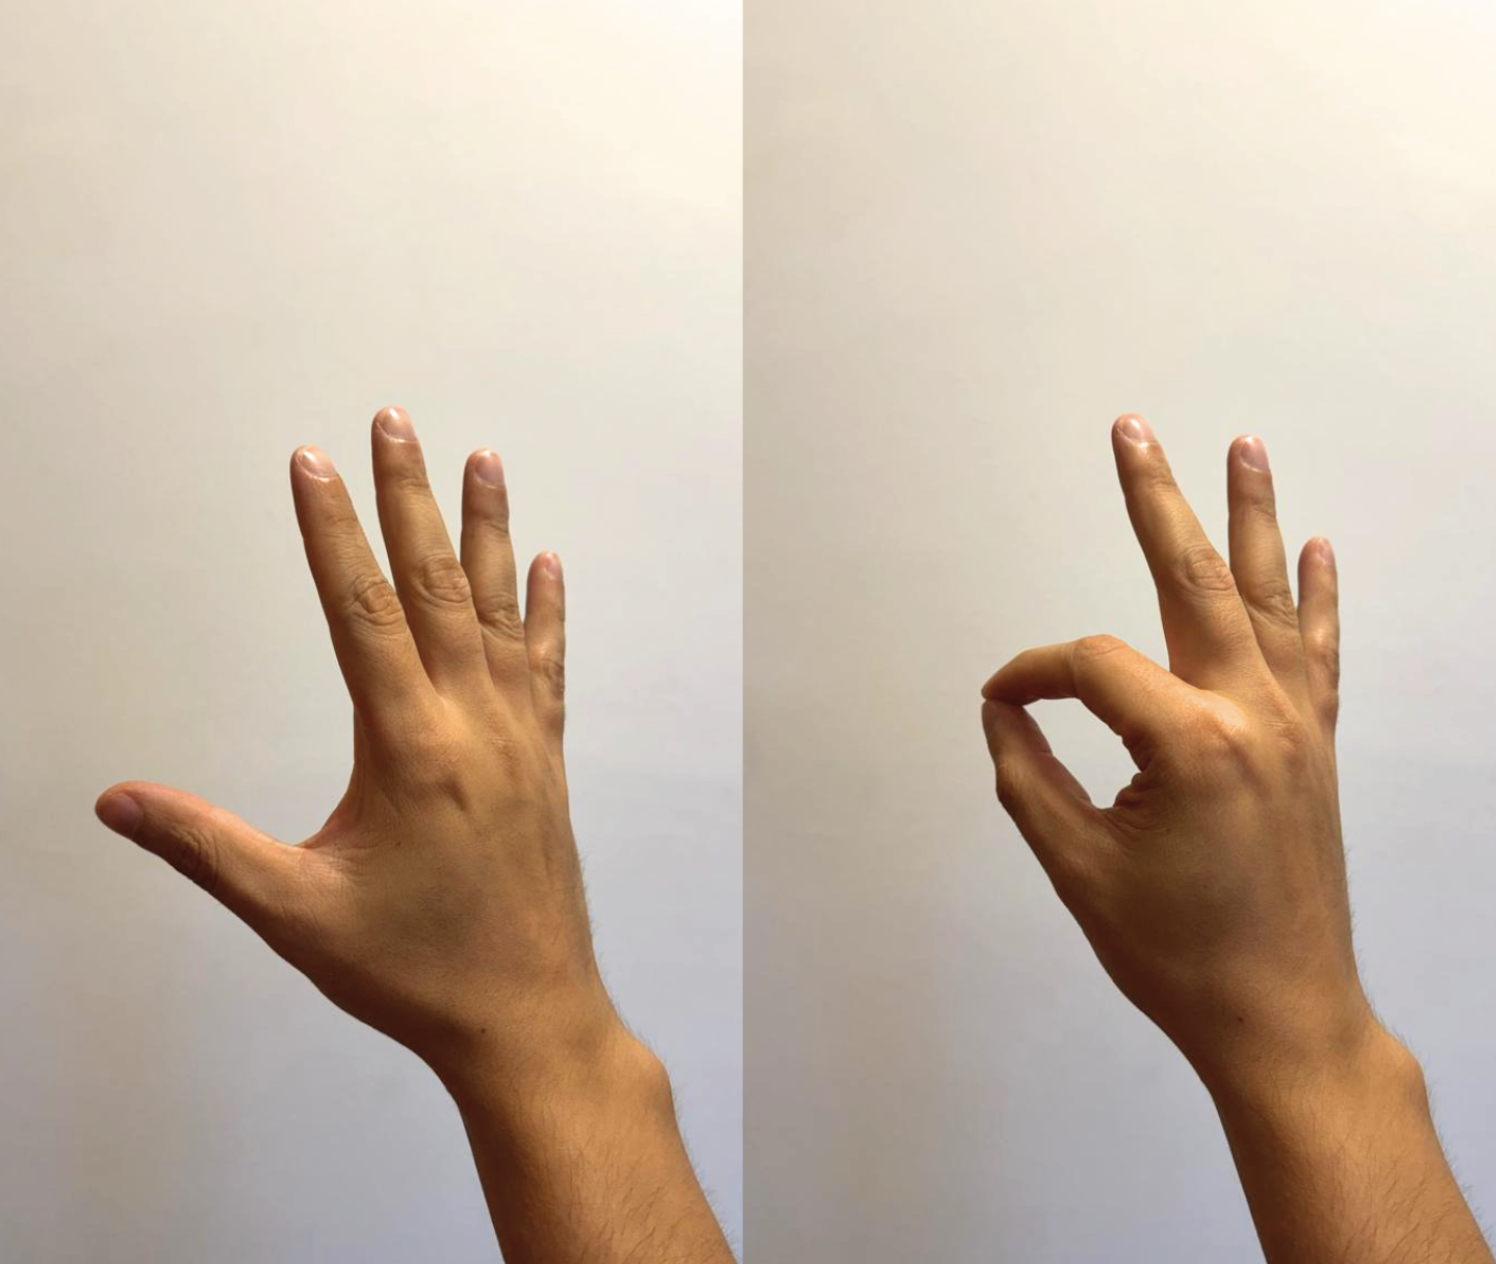
\includegraphics[width=0.88\textwidth]{Figures/cap_1/finger_tapping.png}
	\captionof{figure}{Ejercicio de finger tapping utilizado en la evaluación clínica de movimientos finos de la mano.}
	\label{fig:concepto-finger-tapping}
\end{center}
\vspace{0.4em}

En la figura \ref{fig:concepto-hand-tremor} se ilustra la evaluación del temblor de mano (hand tremor). En ella se observa a una persona de costado con los brazos extendidos hacia el frente, postura utilizada para evaluar los temblores posturales de las extremidades superiores.

\vspace{0.6em}
\begin{center}
	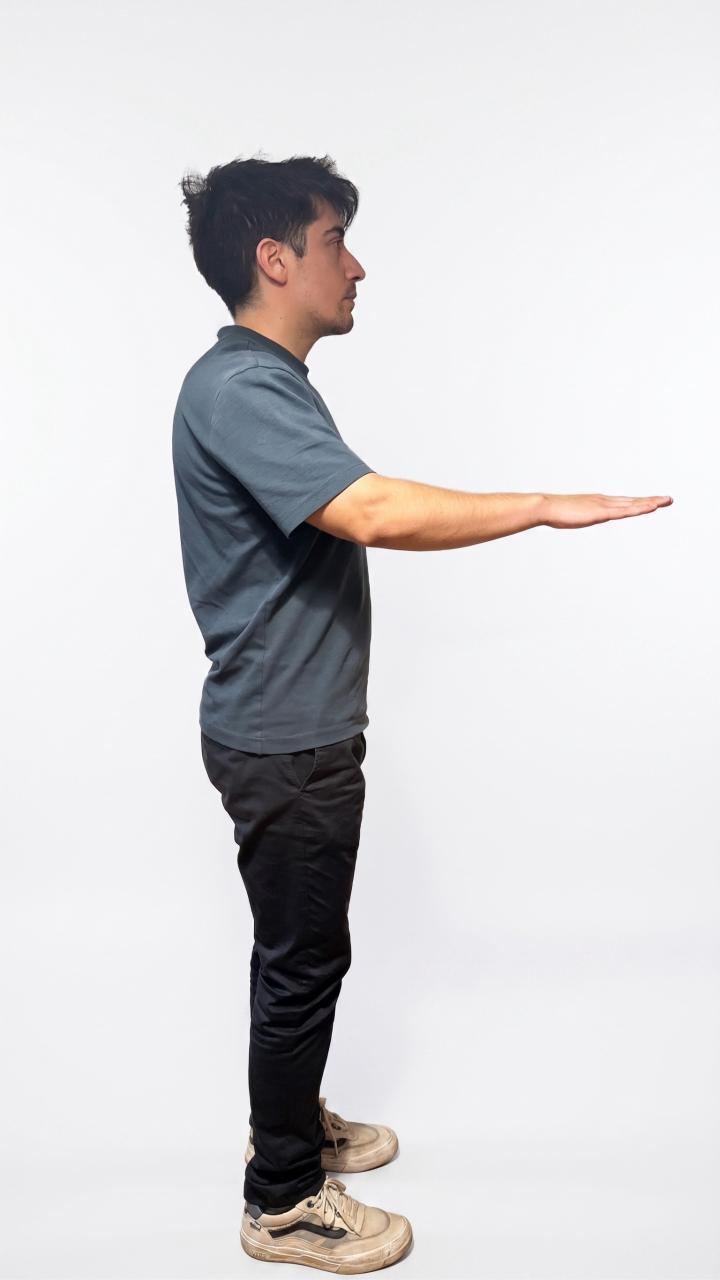
\includegraphics[width=0.34\textwidth]{Figures/cap_1/hand_tremor.jpeg}
	\captionof{figure}{Postura de brazos extendidos hacia el frente para la evaluación del temblor de mano.}
	\label{fig:concepto-hand-tremor}
\end{center}
\vspace{0.4em}

En la figura \ref{fig:concepto-nose-finger} se detalla la prueba nariz-dedo (nose-finger). La secuencia consta de 4 imágenes: inicia con los brazos extendidos, continúa cuando el paciente se toca la nariz con el índice de una mano, vuelve a la postura inicial con ambos brazos extendidos y finaliza cuando se toca la nariz con el índice de la otra mano. Este ejercicio evalúa la precisión del alcance y la coordinación.

\vspace{0.6em}
\begin{center}
	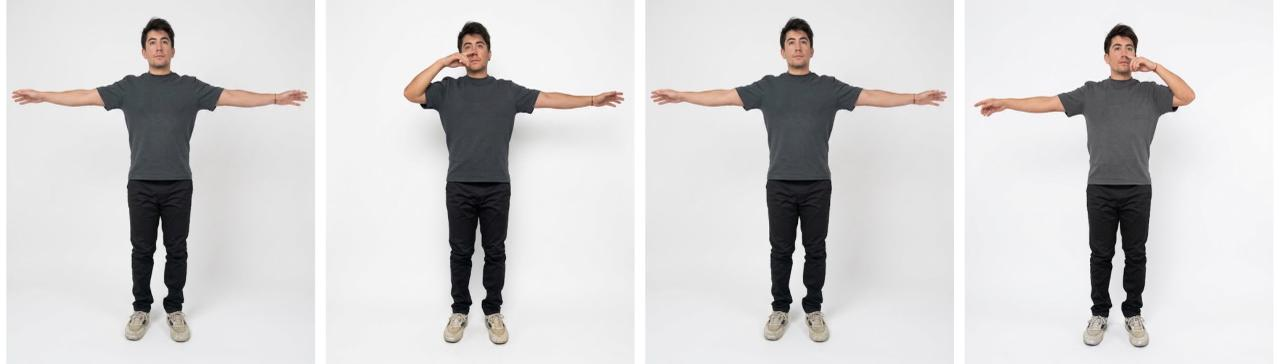
\includegraphics[width=1\textwidth]{Figures/cap_1/nose_finger.jpeg}
	\captionof{figure}{Secuencia de la prueba nariz-dedo, desde la postura de brazos extendidos alternando el contacto con la nariz.}
	\label{fig:concepto-nose-finger}
\end{center}
\vspace{0.4em}

Por último, en la figura \ref{fig:concepto-open-close} se exhibe el ejercicio de apertura y cierre de manos (open-close hands). En la imagen se aprecian las manos de una persona al realizar el ciclo de apertura y cierre. Este ejercicio suele evaluarse en una postura similar a la del temblor de mano, de pie y con los brazos estirados hacia el frente, para analizar la amplitud, la frecuencia y la velocidad de los movimientos.

\vspace{0.6em}
\begin{center}
	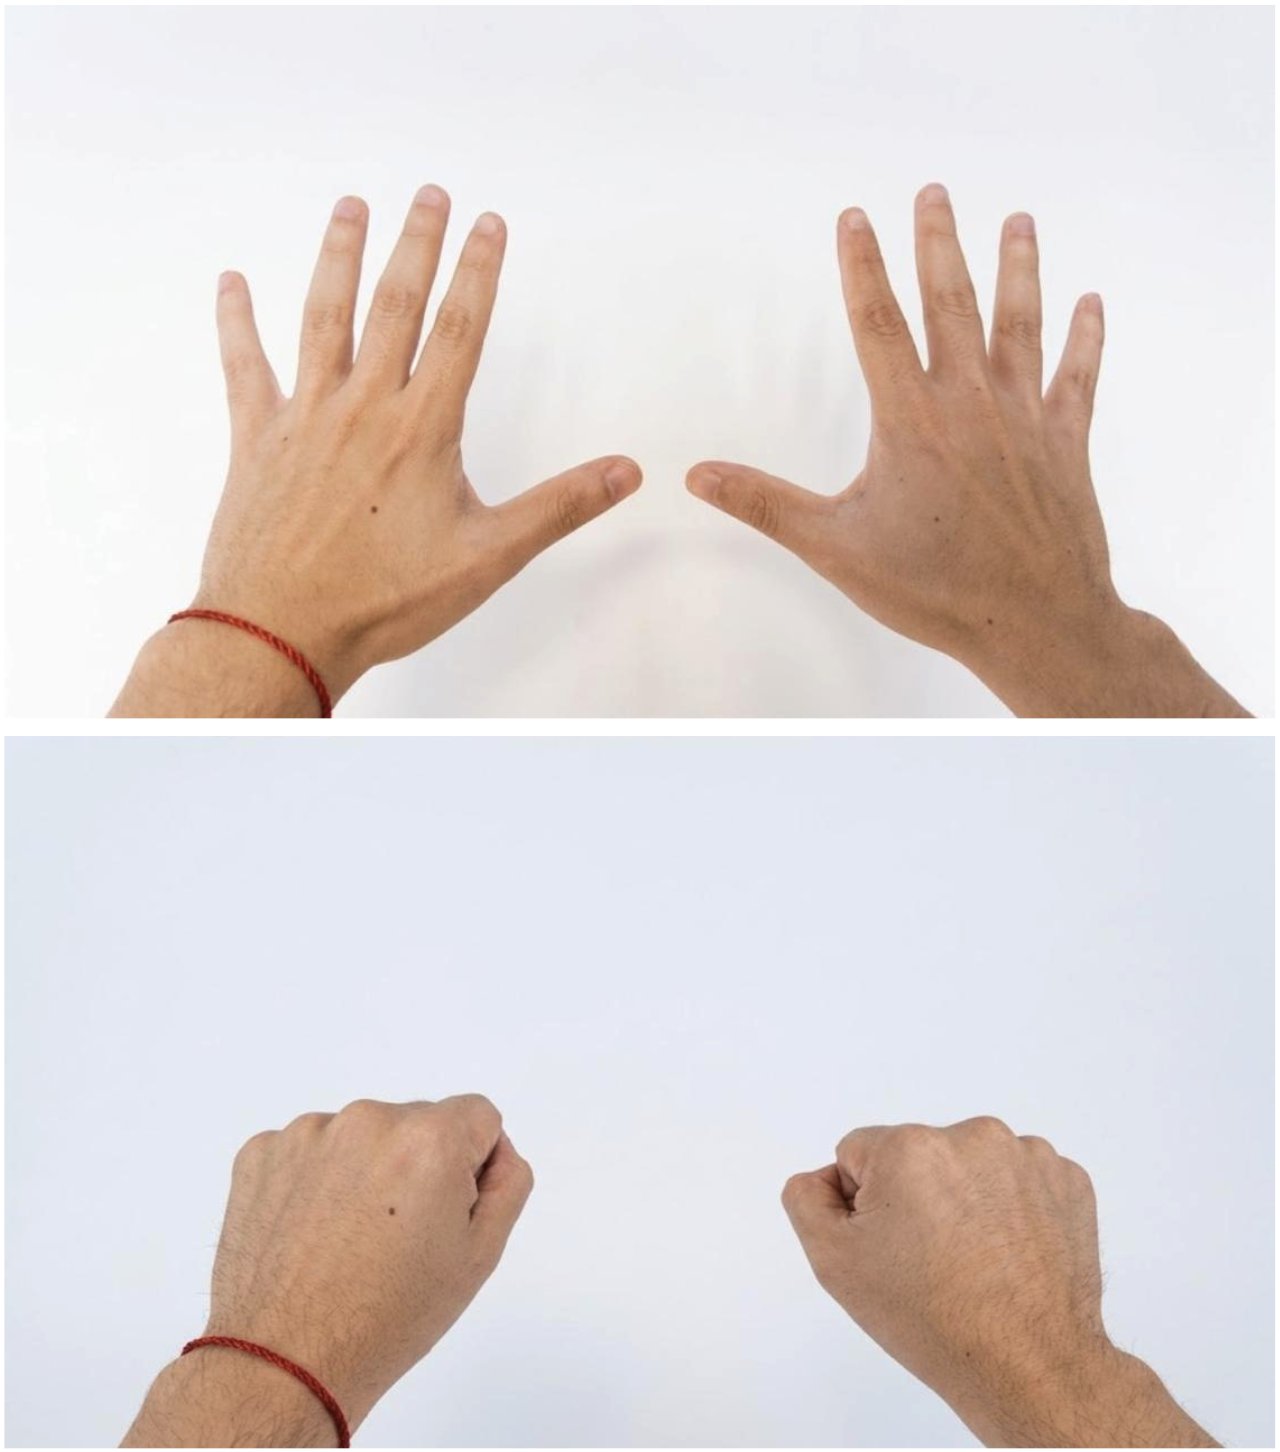
\includegraphics[width=0.54\textwidth]{Figures/cap_1/open_close.png}
	\captionof{figure}{Ejercicio de apertura y cierre de manos, evaluado frecuentemente con los brazos estirados hacia el frente.}
	\label{fig:concepto-open-close}
\end{center}
\vspace{0.4em}

Estas secuencias pueden registrarse en video para analizarlas de forma cuantitativa con herramientas de visión por computadora, como se desarrolla en los capítulos posteriores.

\section{Contexto y motivación}

La motivación del trabajo fue construir una herramienta que, a partir de videos de ejercicios motores, estimara la pose corporal del paciente y derivara métricas asociadas a oscilaciones y regularidad del movimiento. De este modo, se buscó reducir la dependencia exclusiva de la impresión visual humana para apreciar cambios leves o graduales.

La inteligencia artificial y la visión por computadora resultaron adecuadas porque permiten procesar cada fotograma de manera uniforme, conservar el detalle temporal entre cuadros consecutivos y transformar coordenadas articulares en magnitudes interpretables por el personal de salud. Se priorizó un enfoque basado en modelos preentrenados de estimación de pose, alineado con el alcance acordado para el proyecto, que explícitamente no incluyó entrenar redes neuronales desde cero en un conjunto propio de gran escala.

El trabajo culminó con un producto operativo que puede ejecutarse en entorno local y mediante contenedores, y además se desplegó en la nube sobre Google Cloud Platform (GCP) \citep{gcp}, de modo que el acceso al sistema no se limitó a una única máquina de desarrollo. La arquitectura y el procedimiento de despliegue quedaron documentados para facilitar extensiones posteriores, como validación prospectiva frente a lecturas de referencia o adaptaciones institucionales sujetas a marcos éticos y regulatorios propios de cada jurisdicción.

\section{Estado del arte}

La revisión sistemática de Pecoraro, Marsili, Espay, Bologna y di Biase sobre tecnologías de visión por computadora en trastornos del movimiento resume decenas de estudios entre 1984 y 2024 \citep{pecoraro2025computer}. En ese conjunto de investigaciones predominan trabajos sobre la enfermedad de Parkinson y tareas de marcha. Para la estimación de pose sin marcadores físicos aparecen con frecuencia implementaciones basadas en OpenPose \citep{cao2019openpose} y, en menor medida, otras soluciones mediante modelos propios o integraciones desarrolladas para cada estudio.

Los autores destacan que el análisis automático de video alcanzó en muchos informes exactitudes diagnósticas superiores al 80\% frente a etiquetas clínicas, con buena concordancia frente a acelerometría en temblor y distonía, aunque advierten heterogeneidad en condiciones de grabación y en el software empleado, lo que dificulta comparar resultados entre sitios.

En paralelo, el trabajo de Sibley, Girges, Hoque y Foltynie analiza retos metodológicos del análisis de video para cuantificar la severidad motora en Parkinson y el papel de la inteligencia artificial y el aprendizaje automático en ese escenario \citep{sibley2021video}. Concluyen que la evaluación por video es accesible y prometedora, pero que hacen falta muestras amplias y diversas y estándares de desempeño alineados con la práctica clínica antes de generalizar su uso.

Para la estimación de pose en tiempo casi real sobre hardware común, Google publicó el marco MediaPipe, que permite encadenar módulos de visión reutilizables y ajustar el consumo de recursos según el equipo disponible \citep{lugaresi2019mediapipe}. Dentro de ese ecosistema, el modelo de pose corporal ofrece coordenadas normalizadas de puntos anatómicos en dos y tres dimensiones y se utiliza en prototipos de salud y deporte por su equilibrio entre latencia y precisión aceptable para seguimiento de extremidades.

Entre las implementaciones recientes con fines clínicos y de investigación, VisionMD constituyó una plataforma de código abierto destinada al análisis automático de videos de tareas de la parte III de la escala MDS-UPDRS \citep{acevedo2025visionmd}. Mediante aprendizaje profundo localizó al sujeto, permitió marcar con precisión de fotograma el inicio y el fin de cada prueba y derivó variables cinemáticas como amplitud, velocidad y variabilidad a partir del seguimiento markerless de mano y cuerpo con el marco MediaPipe \citep{acevedo2025visionmd,lugaresi2019mediapipe}. El procesamiento se ejecutó en equipos convencionales sin requerir hardware especializado ni envío obligatorio de los videos a servicios en la nube, en contraste con plataformas comerciales cerradas señaladas en la misma publicación.

En estudios piloto con pacientes con enfermedad de Parkinson, los autores reportaron diferencias significativas en métricas de tapping de dedos y otras tareas frente a estados de estimulación cerebral profunda encendida o apagada y frente a niveles de medicación, junto con concordancia inter-evaluador elevada en el uso de la herramienta \citep{acevedo2025visionmd}. Ese trabajo ilustró la viabilidad de cuantificar de forma objetiva pruebas ya incorporadas a la exploración motora estandarizada.

En diciembre del año 2025, como extensión de la plataforma VisionMD, Guarín presentó un método para cuantificar la amplitud y frecuencia del temblor postural de la mano directamente desde videos de teléfonos inteligentes, sin requerir referencias de calibración externas \citep{guarin2025postural}. La propuesta combinó la estimación del diámetro del iris para establecer una escala métrica con modelos de estimación de pose 3D y seguimiento de manos, logrando una fuerte correlación con las puntuaciones clínicas tradicionales y sensibilidad a los efectos del tratamiento.

El prototipo documentado en esta memoria se inscribió en la misma línea de visión sin marcadores físicos basada en MediaPipe Pose y en el análisis de tareas motoras finas a partir de series de puntos clave, pero priorizó un flujo operativo orientado a servicios y despliegue mediante contenedores, como se describe en los capítulos siguientes.

En la tabla \ref{tab:comparativa-enfoques} se contrastan enfoques representativos del estado del arte en cuanto a insumos, salida típica y forma habitual de evaluación reportada en la literatura de revisión. No constituye un inventario exhaustivo de productos comerciales sino una guía conceptual para situar el trabajo desarrollado.

\vspace{0.6em}
\begin{center}
\begin{minipage}{\textwidth}
\centering
\captionof{table}{Enfoques frecuentes para cuantificar el movimiento en Parkinson y contextos afines.}
\label{tab:comparativa-enfoques}
{\setlength{\tabcolsep}{3.5pt}\small
\begin{tabular}{@{}p{0.20\textwidth}p{0.23\textwidth}p{0.26\textwidth}p{0.23\textwidth}@{}}
\toprule
\tabhead{Enfoque} & \tabhead{Datos de entrada} & \tabhead{Salida típica} & \tabhead{Evaluación habitual en la literatura} \\
\midrule
Escalas clínicas (MDS-UPDRS III y otras). & Observación en vivo o video asistido por humano. & Puntuaciones ordinales por ítem. & Consistencia inter-examinador, validez frente a estándares clínicos. \\
Sensores inerciales. & Aceleración o velocidad angular en segmentos corporales. & Series temporales, estimadores de frecuencia y amplitud. & Concordancia con video o con escala clínica. \\
OpenPose u otras redes de pose markerless. & Video monocular o multivista. & Coordenadas 2D o 3D de articulaciones. & Exactitud de clasificación o correlación con medidas de referencia \citep{pecoraro2025computer}. \\
MediaPipe Pose. & Video; modelos preentrenados integrados al marco. & Landmarks normalizados 2D/3D y continuidad temporal en un grafo de procesamiento integrado \citep{lugaresi2019mediapipe}. & Idoneidad para tiempo casi real y bajo consumo en dispositivos habituales, frente a estimadores más pesados \citep{lugaresi2019mediapipe}. \\
\bottomrule
\end{tabular}}
\end{minipage}
\end{center}
\vspace{0.4em}

\section{Objetivos del trabajo}

Con el contexto clínico, la motivación del análisis automático de video y el panorama de la literatura ya expuestos, a continuación se enuncian el objetivo general y los objetivos específicos que guiaron el desarrollo del sistema.

\subsection{Objetivo general}

Diseñar e implementar un sistema de análisis digital de oscilaciones y desempeño motor en videos de ejercicios clínicos asociados a la enfermedad de Parkinson, apoyado en estimación automática de pose y en técnicas de procesamiento de señales e inteligencia artificial, que entregue métricas cuantitativas y visualizaciones comprensibles para apoyar el seguimiento objetivo del movimiento.

\subsection{Objetivos específicos}

\begin{enumerate}
\item Implementar un flujo de ingesta y preprocesamiento de video que alimente de manera estable el estimador de pose y módulos posteriores.
\item Integrar un modelo preentrenado de estimación de pose corporal y un seguimiento temporal de puntos relevantes para los ejercicios considerados.
\item Calcular métricas de amplitud, frecuencia, regularidad y estabilidad postural, u otras derivadas del mismo principio de análisis de series articulares, y agregarlas por sesión para su revisión estadística.
\item Exponer los resultados mediante una interfaz de servicios y una aplicación web que permitan cargar sesiones, inspeccionar gráficos y exportar reportes estructurados.
\item Verificar el comportamiento del software mediante pruebas unitarias y de integración sobre componentes críticos del flujo de procesamiento.
\end{enumerate}

Los criterios de cumplimiento asociados a estos objetivos fueron la ejecución exitosa del flujo completo sobre videos de prueba disponibles para el proyecto, la coherencia de las métricas frente a escenarios controlados o simulados descritos en el capítulo de ensayos, y el paso de la batería de pruebas automatizadas definida en el repositorio del sistema.

% Chapter 2

\chapter{Introducción específica} % Main chapter title

\label{Chapter2}

En este capítulo se describen las herramientas, bibliotecas, modelos preentrenados y conjuntos de datos provistos por terceros que sostuvieron el desarrollo del sistema. También se detallan el origen y las características de los videos utilizados y la infraestructura de ejecución contemplada para los ensayos y para el despliegue del prototipo.

%----------------------------------------------------------------------------------------

\section{Frameworks y bibliotecas}
\label{sec:frameworks}

El sistema se construyó sobre tecnologías de código abierto. El núcleo del trabajo es un flujo de procesamiento de video y señales escrito en \texttt{Python} 3.12, sobre el que se montan un servicio HTTP, una capa de persistencia y una interfaz web. Esta separación permitió que la misma lógica de procesamiento se pudiera invocar desde una línea de comandos, desde un servicio HTTP o desde un contenedor sin alterar el núcleo del cálculo.

Para la lectura y manipulación de imagen se utilizó \texttt{OpenCV} \citep{bradski2000opencv}, que cubrió la apertura de los archivos de video, la conversión entre espacios de color y las operaciones de redimensionado y muestreo cuadro a cuadro. La extracción del canal de audio asociado a las grabaciones se realizó con \texttt{moviepy}, y el análisis posterior de ese canal, en particular para la detección de los pulsos del metrónomo que estructuran los ejercicios, se apoyó en \texttt{librosa} \citep{mcfee2015librosa}, una biblioteca especializada en el procesamiento de señales de audio musicales y rítmicas.

El cálculo de las métricas se sostuvo en el conjunto de bibliotecas científicas habituales del ecosistema \texttt{Python}, integrado por \texttt{NumPy}, \texttt{SciPy} y \texttt{pandas} \citep{virtanen2020scipy}. \texttt{NumPy} proveyó las operaciones vectoriales sobre las series temporales de los puntos detectados, \texttt{SciPy} aportó los estimadores espectrales y los algoritmos de detección de picos utilizados para el cálculo de frecuencia y de regularidad, y \texttt{pandas} se utilizó para organizar los datos por cuadro en estructuras tabulares que luego alimentan los pasos de agregación y exportación.

La capa de servicios se desarrolló con \texttt{FastAPI} \citep{fastapi}, un \textit{framework} para servicios HTTP en \texttt{Python} con soporte nativo para validación de datos a través de \texttt{Pydantic}, generación automática de documentación interactiva y eventos de servidor (\textit{server-sent events}) que se utilizaron para informar el progreso de cada análisis en tiempo casi real. La persistencia de pacientes, sesiones y resultados quedó a cargo de \texttt{PostgreSQL} \citep{postgresql}, una base de datos relacional de uso amplio en aplicaciones de producción, accedida desde la aplicación mediante el \textit{object-relational mapper} \texttt{SQLAlchemy} y administrada mediante \texttt{Alembic} para el versionado del esquema.

La interfaz de usuario se construyó como una aplicación web de página única en \texttt{TypeScript}, con un conjunto estándar de bibliotecas para componentes visuales, ruteo y gráficos interactivos. El detalle de esa capa se desarrolla en el capítulo de diseño e implementación, donde resulta más pertinente describir la arquitectura del frontend.

En el plano de operación y empaquetado se adoptaron \texttt{Docker} \citep{merkel2014docker} y \texttt{Docker Compose} para orquestar la base de datos, el servicio HTTP y el sirviente de contenido estático en una topología única que se reproduce de igual manera en el entorno local y en el destino de despliegue. Las dependencias de \texttt{Python} se gestionaron con \texttt{uv}, mientras que la calidad del código se verificó mediante análisis estático y un conjunto de pruebas automatizadas con \texttt{pytest}.

En la tabla \ref{tab:bibliotecas-cap2} se sintetizan las bibliotecas y herramientas más relevantes para el procesamiento de datos y para el funcionamiento del sistema, agrupadas por su rol y con la motivación principal de su elección.

\vspace{0.6em}
\begin{center}
\begin{minipage}{\textwidth}
\centering
\captionof{table}{Bibliotecas y herramientas de terceros utilizadas en el desarrollo del sistema, agrupadas por capa funcional.}
\label{tab:bibliotecas-cap2}
\begin{tabular}{p{3.2cm}p{4.2cm}p{6.2cm}}
\toprule
\tabhead{Capa} & \tabhead{Herramientas} & \tabhead{Motivo de elección} \\
\midrule
Visión y video & MediaPipe, OpenCV & Modelos preentrenados de pose listos para uso y manipulación robusta de archivos de video. \\
Audio & librosa, moviepy & Extracción del canal de audio y detección de pulsos rítmicos para los ejercicios con metrónomo. \\
Numérica y métricas & NumPy, SciPy, pandas & Operaciones vectoriales, estimadores espectrales y manipulación tabular ampliamente probadas. \\
Servicios HTTP & FastAPI, Pydantic & Validación de datos integrada y soporte nativo para flujos de progreso por SSE. \\
Persistencia & PostgreSQL, SQLAlchemy, Alembic & Base relacional madura, ORM y versionado declarativo del esquema. \\
Modelo de lenguaje & OpenAI Python SDK & Acceso a un modelo de lenguaje generativo para resúmenes interpretativos de las sesiones. \\
Operación & Docker, Docker Compose, uv & Despliegue equivalente en local y nube y dependencias reproducibles. \\
\bottomrule
\end{tabular}
\end{minipage}
\end{center}
\vspace{0.4em}

La elección de tecnologías favoreció componentes de uso difundido y bien documentados, lo que se alineó con los supuestos del proyecto sobre disponibilidad de bibliotecas de código abierto y contribuyó a mitigar el riesgo identificado en la planificación inicial respecto a posibles incompatibilidades en la integración de modelos de visión por computadora.

\section{Datasets y datos}
\label{sec:datasets}

El trabajo no contempló el entrenamiento de modelos desde cero, por lo que las necesidades de datos se concentraron en disponer de una cantidad de video suficiente para verificar la integración del flujo de procesamiento, evaluar la coherencia de las métricas en escenarios reproducibles y exponer la herramienta a movimientos representativos de los ejercicios contemplados.

No se incorporaron conjuntos de datos públicos. La conformación de un conjunto de grabaciones de pacientes con enfermedad de Parkinson exige un marco de consentimiento informado, anonimización y resguardo bajo regulaciones de protección de datos de salud, condiciones que se inscriben en una etapa posterior a la de un prototipo de investigación. Esa restricción se reflejó desde la planificación inicial, que excluyó explícitamente del alcance la validación clínica formal y la integración con sistemas hospitalarios y dejó la evaluación funcional con especialistas como actividad opcional. En el desarrollo se realizó además un análisis preliminar de los principales puntos de mejora y de criticidad para que el sistema pueda alinearse con normativas vigentes de protección de datos sanitarios, como la \textit{Health Insurance Portability and Accountability Act} (HIPAA) en su jurisdicción de origen. El resultado de ese análisis y las propuestas asociadas se desarrollan en los capítulos posteriores como trabajo futuro y propuestas de mejora.

Para sostener el avance del desarrollo dentro del alcance descripto, se trabajó con dos fuentes complementarias de video: grabaciones propias de personas sanas que reprodujeron los ejercicios estandarizados y un conjunto reducido de grabaciones de pacientes obtenidas en condiciones controladas y bajo acuerdo de uso interno, que se mantuvieron por fuera del repositorio de código.

Esta estrategia resultó adecuada para los objetivos del trabajo porque el sistema se apoya en modelos preentrenados de estimación de pose, cuya capacidad de detectar puntos anatómicos no depende del diagnóstico de la persona registrada. Las grabaciones de personas sanas resultaron suficientes para verificar la robustez del seguimiento de \textit{keypoints} bajo distintos encuadres y condiciones de iluminación, mientras que las grabaciones de pacientes permitieron observar el comportamiento del sistema en presencia de los patrones motores característicos. La ampliación posterior del conjunto con material clínico anotado se identificó como una línea natural de continuidad y se desarrolla en el capítulo de conclusiones.

Las grabaciones se obtuvieron con la cámara posterior de un teléfono \textit{iPhone} 15 Pro a 30 cuadros por segundo, en disposición fija sobre una superficie plana y con la región de interés (mano dominante o tronco superior, según el ejercicio) centrada en el cuadro. Durante los primeros segundos de cada grabación se ubicó en el campo visual un tablero de calibración \textit{ChArUco} \citep{garrido2014charuco}, que el sistema utiliza para estimar la conversión píxeles–milímetros sin requerir intervención manual del operador. En la tabla \ref{tab:videos-cap2} se resumen las características del conjunto de grabaciones utilizado, según la fuente de los videos y el ejercicio principal asociado a cada grupo.

\vspace{0.6em}
\begin{center}
\begin{minipage}{\textwidth}
\centering
\captionof{table}{Caracterización resumida del conjunto de grabaciones de video utilizado en el desarrollo y la verificación del sistema.}
\label{tab:videos-cap2}
\begin{tabular}{p{3.6cm}p{3.8cm}p{6.0cm}}
\toprule
\tabhead{Fuente} & \tabhead{Ejercicios cubiertos} & \tabhead{Notas de captura} \\
\midrule
Grabaciones propias de personas sanas & \textit{Finger tapping}, temblor de mano, oscilación de brazos & Cámara fija, iluminación ambiente, tablero de calibración al inicio. \\
Grabaciones reducidas de pacientes & \textit{Finger tapping}, dedo a nariz & Obtenidas bajo acuerdo de uso interno, almacenadas por fuera del repositorio. \\
Material de muestra anonimizado & \textit{Finger tapping}, ejercicios de demostración & Incluido en el repositorio para pruebas de integración continua y para la incorporación de nuevos colaboradores. \\
\bottomrule
\end{tabular}
\end{minipage}
\end{center}
\vspace{0.4em}

El conjunto se administró bajo una clasificación de tres niveles definida en el repositorio del sistema: material de muestra anonimizado, grabaciones reales de pacientes y artefactos de salida del análisis, con políticas explícitas de almacenamiento y de exclusión del control de versiones para los dos últimos. Esa política se documentó internamente para evitar la difusión accidental de datos sensibles y se alinea con los requerimientos éticos enunciados en la planificación inicial.

\section{Modelos preentrenados}
\label{sec:modelos-preentrenados}

Una de las decisiones de alcance establecidas al inicio del trabajo fue no entrenar redes neuronales desde cero, sino apoyarse en modelos preentrenados de uso difundido. Esa decisión se fundamentó en el equilibrio entre el costo de obtener un conjunto etiquetado de gran tamaño y la disponibilidad de soluciones maduras para la estimación de pose de mano y de cuerpo completo, ya validadas en aplicaciones de salud, deporte y realidad aumentada.

Para la estimación de pose se utilizaron dos modelos del marco \texttt{MediaPipe} \citep{lugaresi2019mediapipe}, distribuidos a través de la API de tareas (\textit{Tasks API}) en su versión 0.10. El modelo \texttt{HandLandmarker} \citep{zhang2020mediapipehands} entrega 21 puntos por mano detectada, organizados en falanges y articulaciones, y se utilizó en todos los ejercicios centrados en la mano. El modelo \texttt{PoseLandmarker} en su variante \textit{lite} \citep{bazarevsky2020blazepose} entrega 33 puntos del cuerpo y se reservó para los ejercicios que requerían el contexto del torso y los brazos. Ambos modelos se descargaron desde el repositorio público de \texttt{MediaPipe} en formato \textit{float16} y se almacenaron localmente en una caché versionada de modelos.

En la figura \ref{fig:mediapipe-hand-cap2} se muestra un ejemplo de los 21 puntos de referencia entregados por el modelo \texttt{HandLandmarker}, ubicados sobre la imagen de una mano en la postura típica del ejercicio de \textit{finger tapping}.

\vspace{0.6em}
\begin{center}

\includegraphics[width=0.7\textwidth]{Figures/cap_2/placeholder_mediapipe_hand.png}
\captionof{figure}{Ejemplo ilustrativo de los puntos de referencia entregados por el modelo \texttt{HandLandmarker} de \texttt{MediaPipe} sobre la imagen de una mano. Imagen pendiente de reemplazo por una visualización propia generada con el sistema.}
\label{fig:mediapipe-hand-cap2}
\end{center}
\vspace{0.4em}

En la imagen se observa la disposición regular de los puntos a lo largo de las falanges y las articulaciones, que permite reconstruir la geometría de la mano cuadro a cuadro y, a partir de ella, derivar las distancias y los ángulos sobre los que se calculan las métricas del sistema.

Para la generación automática de resúmenes interpretativos sobre los resultados de cada sesión y sobre la evolución longitudinal de un paciente se incorporó un modelo de lenguaje de gran tamaño (\textit{large language model}, LLM), accedido a través de la API de OpenAI \citep{openai_api}. El modelo elegido fue \texttt{GPT-5.4-mini}, una variante orientada a tareas conversacionales con costo y latencia acotados. El componente del sistema responsable de esta funcionalidad envía únicamente las métricas cuantitativas y los metadatos no identificatorios de la sesión, junto con un conjunto acotado de instrucciones en formato \textit{prompt} estructurado, y recibe un texto en lenguaje natural que el profesional de salud puede inspeccionar como apoyo a la lectura del reporte. El modelo nunca recibe identificadores del paciente, en línea con la política de manejo de datos del proyecto.

En la tabla \ref{tab:modelos-cap2} se sintetizan los modelos preentrenados utilizados, indicando su origen, la tarea sobre la que operan y las características relevantes para el sistema.

\vspace{0.6em}
\begin{center}
\begin{minipage}{\textwidth}
\centering
\captionof{table}{Modelos preentrenados de terceros incorporados al sistema.}
\label{tab:modelos-cap2}
\begin{tabular}{p{3cm}p{3cm}p{3.6cm}p{3.6cm}}
\toprule
\tabhead{Modelo} & \tabhead{Tarea} & \tabhead{Origen y datos de preentrenamiento} & \tabhead{Uso en el sistema} \\
\midrule
HandLandmarker (MediaPipe 0.10) & Detección de 21 puntos por mano & Imágenes anotadas de manos en distintas poses, entornos y condiciones de iluminación \citep{zhang2020mediapipehands} & Ejercicios de \textit{finger tapping} y temblor de mano \\
PoseLandmarker Lite (MediaPipe 0.10) & Detección de 33 puntos corporales & Imágenes y video con anotaciones de pose corporal completa \citep{bazarevsky2020blazepose} & Ejercicios con contexto de tronco y brazos \\
GPT-5.4-mini (OpenAI) & Modelo de lenguaje generativo & Conjunto general empleado por OpenAI para sus modelos de propósito general \citep{openai_api} & Resúmenes interpretativos por sesión y por evolución a partir de las métricas calculadas \\
\bottomrule
\end{tabular}
\end{minipage}
\end{center}
\vspace{0.4em}

La integración de los modelos respetó los supuestos del proyecto sobre acceso a soluciones de código abierto y la decisión explícita de no entrenar desde cero. De ese modo se concentró el esfuerzo en el flujo de procesamiento, en la derivación de métricas y en la presentación clínica de los resultados, en lugar de en la construcción de un \textit{dataset} de entrenamiento y de un protocolo de ajuste de redes neuronales. Otro aporte significativo del trabajo fue la operación e integración de los servicios necesarios para conformar una solución completa, que articula la infraestructura de ejecución, la interfaz de usuario, el servicio de aplicación y la persistencia en una arquitectura coherente y reproducible, descripta en el capítulo de diseño e implementación.

\section{Infraestructura}
\label{sec:infraestructura}

% NOTA: sección iniciada en una primera iteración. El detalle del despliegue
% en GCP, la decisión sobre uso de GPU o solo CPU para la inferencia y la
% caracterización del equipo local de desarrollo se completarán en una
% iteración posterior.

\textit{[Sección en elaboración. Se completará en una segunda iteración.]}

El sistema se diseñó para ejecutarse de manera equivalente en una máquina de desarrollo local y en un entorno desplegado en la nube, condición incluida explícitamente como requerimiento de interoperabilidad en la planificación inicial. Para sostener esa equivalencia, todas las dependencias se empaquetaron en imágenes de contenedor reproducibles mediante \texttt{Docker} y se orquestaron a través de \texttt{Docker Compose}, que coordina el servicio de base de datos, el servicio HTTP y el sirviente de contenido estático en una topología única. La configuración sensible al entorno se externalizó en variables de entorno con prefijo \texttt{DAGO\_}, lo que evitó la dependencia de rutas o credenciales fijadas en el código fuente.

Como destino de despliegue para el prototipo se contempló \textit{Google Cloud Platform} (GCP), seleccionado por su disponibilidad de servicios gestionados de cómputo y de almacenamiento compatibles con la topología de contenedores adoptada. La descripción precisa del servicio empleado, el dimensionamiento de las instancias y el manejo del almacenamiento de los videos cargados se desarrollarán en la segunda iteración de este capítulo, junto con la caracterización del equipo de desarrollo local sobre el que se realizó la implementación y la justificación de la inferencia exclusivamente en CPU para los modelos de pose.

% Chapter 3

\chapter{Diseño e implementación}

\label{Chapter3}

En este capítulo se describen los criterios de diseño del sistema, el flujo de procesamiento de video desde la ingesta hasta la exportación de métricas, la arquitectura analítica, la orquestación de inferencia y el cálculo de métricas, y el desarrollo de la aplicación web con su despliegue. Las bibliotecas, modelos y servicios de terceros ya presentados en el capítulo anterior se asumen como base tecnológica y aquí se detalla cómo se organizan en módulos propios del trabajo.

%----------------------------------------------------------------------------------------

\section{Pipeline de datos}
\label{sec:pipeline}

El núcleo del sistema se implementó como un paquete \texttt{pipeline} en \texttt{Python}, independiente de la capa HTTP, de modo que el mismo flujo puede ejecutarse desde la línea de comandos o desde el servicio en segundo plano de la API. El diseño priorizó la modularidad por etapas, la reproducibilidad de parámetros mediante configuración centralizada y la calibración automática de escala sin intervención manual del operador cuando el video incluye un tablero ChArUco al inicio de la grabación, tal como se documentó en la sección \ref{sec:datasets}.

\subsection{Ingesta de video y audio}

La etapa de ingesta comienza con \texttt{VideoLoader}, que abre el archivo mediante \texttt{OpenCV}, extrae metadatos (resolución, cuadros por segundo, cantidad de fotogramas) y expone un iterador de fotogramas con muestreo configurable. En paralelo, \texttt{AudioExtractor} decodifica el canal de audio del contenedor de video a una señal monofónica en formato de punto flotante, requisito para detectar los pulsos del metrónomo que estructuran varios protocolos de grabación.

Sobre esa señal se aplica \texttt{detect\_impulses}, que enfatiza el rango de frecuencias configurado (por defecto entre 400 y 7000~Hz), calcula la envolvente y localiza picos con un umbral de prominencia adaptativo basado en el rango intercuartílico de la envolvente. Los instantes detectados se almacenan como eventos de impulso con marca temporal. A partir de ellos, \texttt{estimate\_metronome\_bpm} estima los pulsos por minuto del metrónomo y una medida de confianza derivada de la variabilidad entre intervalos, información que luego se incorpora al resumen de sesión para contextualizar el ritmo esperado del ejercicio.

\vspace{-\parskip}%
\subsection{Preprocesamiento de imagen}

Cada fotograma leído pasa por \texttt{FrameProcessor}, que convierte el espacio de color de BGR a RGB, redimensiona el ancho a un máximo de 640 píxeles cuando el video supera esa resolución y registra indicadores de calidad por cuadro. En el servicio HTTP el procesamiento se ejecuta en modo streaming: se lee un fotograma, se redimensiona, se estima la pose y se descarta el buffer, de modo que no se acumula en la memoria la secuencia completa. Para controlar el costo computacional en videos de 30 ó más cuadros por segundo, el algoritmo de la solución subsamplea la secuencia a un máximo efectivo de 15 cuadros analizados por segundo y calcula el paso entre fotogramas como el cociente entero entre la tasa nominal y ese tope. La tasa efectiva resultante se utiliza en todas las métricas que dependen de la frecuencia de muestreo, en particular el análisis espectral del temblor.

\subsection{Calibración espacial}

Las distancias articulares se expresan preferentemente en milímetros. Para ello, el sistema implementó una estrategia de calibración con alternativas para el uso de un patrón físico impreso o la estimación biométrica sin marcadores.

Cuando el video incluye un tablero impreso al inicio de la grabación, se estima el factor de conversión píxeles a milímetros a partir de detecciones de un tablero ChArUco en una muestra de fotogramas. La geometría del tablero impreso (cuadrícula 5$\times$7, lado de cuadrado 25~mm, marcadores ArUco \texttt{DICT\_4X4\_50}) coincide con la documentación interna del repositorio y con las condiciones de captura descritas en la sección \ref{sec:datasets}. El muestreo de fotogramas para ChArUco se concentra en los primeros 12~s del video, con paso configurable, para privilegiar el intervalo en el que el tablero permanece visible. Cuando la detección de esquinas internas del tablero falla pero los marcadores ArUco individuales son visibles, se aplica un estimador alternativo basado en la longitud conocida del marcador, lo que incrementa la robustez ante oclusión parcial.

Para ejercicios en los que sostener un tablero impreso resulta impracticable, como en la evaluación del temblor de mano (\texttt{hand\_tremor}), se implementó una calibración biométrica sin marcadores. Este método utiliza el ancho promedio del iris humano como referencia métrica conocida en el plano facial. Para trasladar esa escala desde el rostro hasta la mano que experimenta el temblor, se calcula la profundidad absoluta de ambas partes del cuerpo mediante la red neuronal MeTRAbs (del inglés \textit{Metric Scale 3D Human Pose Estimation}) mencionada en la sección \ref{sec:modelos-preentrenados}. Esta combinación permite ajustar el factor de conversión milímetros por píxel en la mano en función de la perspectiva de la cámara. Como medida de contingencia, el sistema conserva una calibración manual heredada (\texttt{legacy}) mediante parámetros de distancia directa en píxeles.

El resultado de la calibración se propaga al seguimiento y queda registrado en el resumen de sesión: método empleado (\texttt{charuco}, \texttt{markerless\_iris\_metrabs} o \texttt{legacy}), milímetros por píxel, tasa de detección, disponibilidad de la estimación de profundidad y parámetros geométricos. Esa trazabilidad permite al operador interpretar si las distancias en milímetros deben tomarse con reserva y habilita la auditoría visual del procedimiento.

En la figura \ref{fig:charuco-overlay} se puede observar un fotograma del video con el tablero detectado para estimar la relación milímetros por píxel. Cada uno de los recuadros verdes representa la detección de los marcadores del tablero. A partir de esa medición en píxeles y al conocer la dimensión real de los marcadores en milímetros, se puede obtener la relación milímetros por píxel buscada.

\begin{figure}[htbp]
\centering
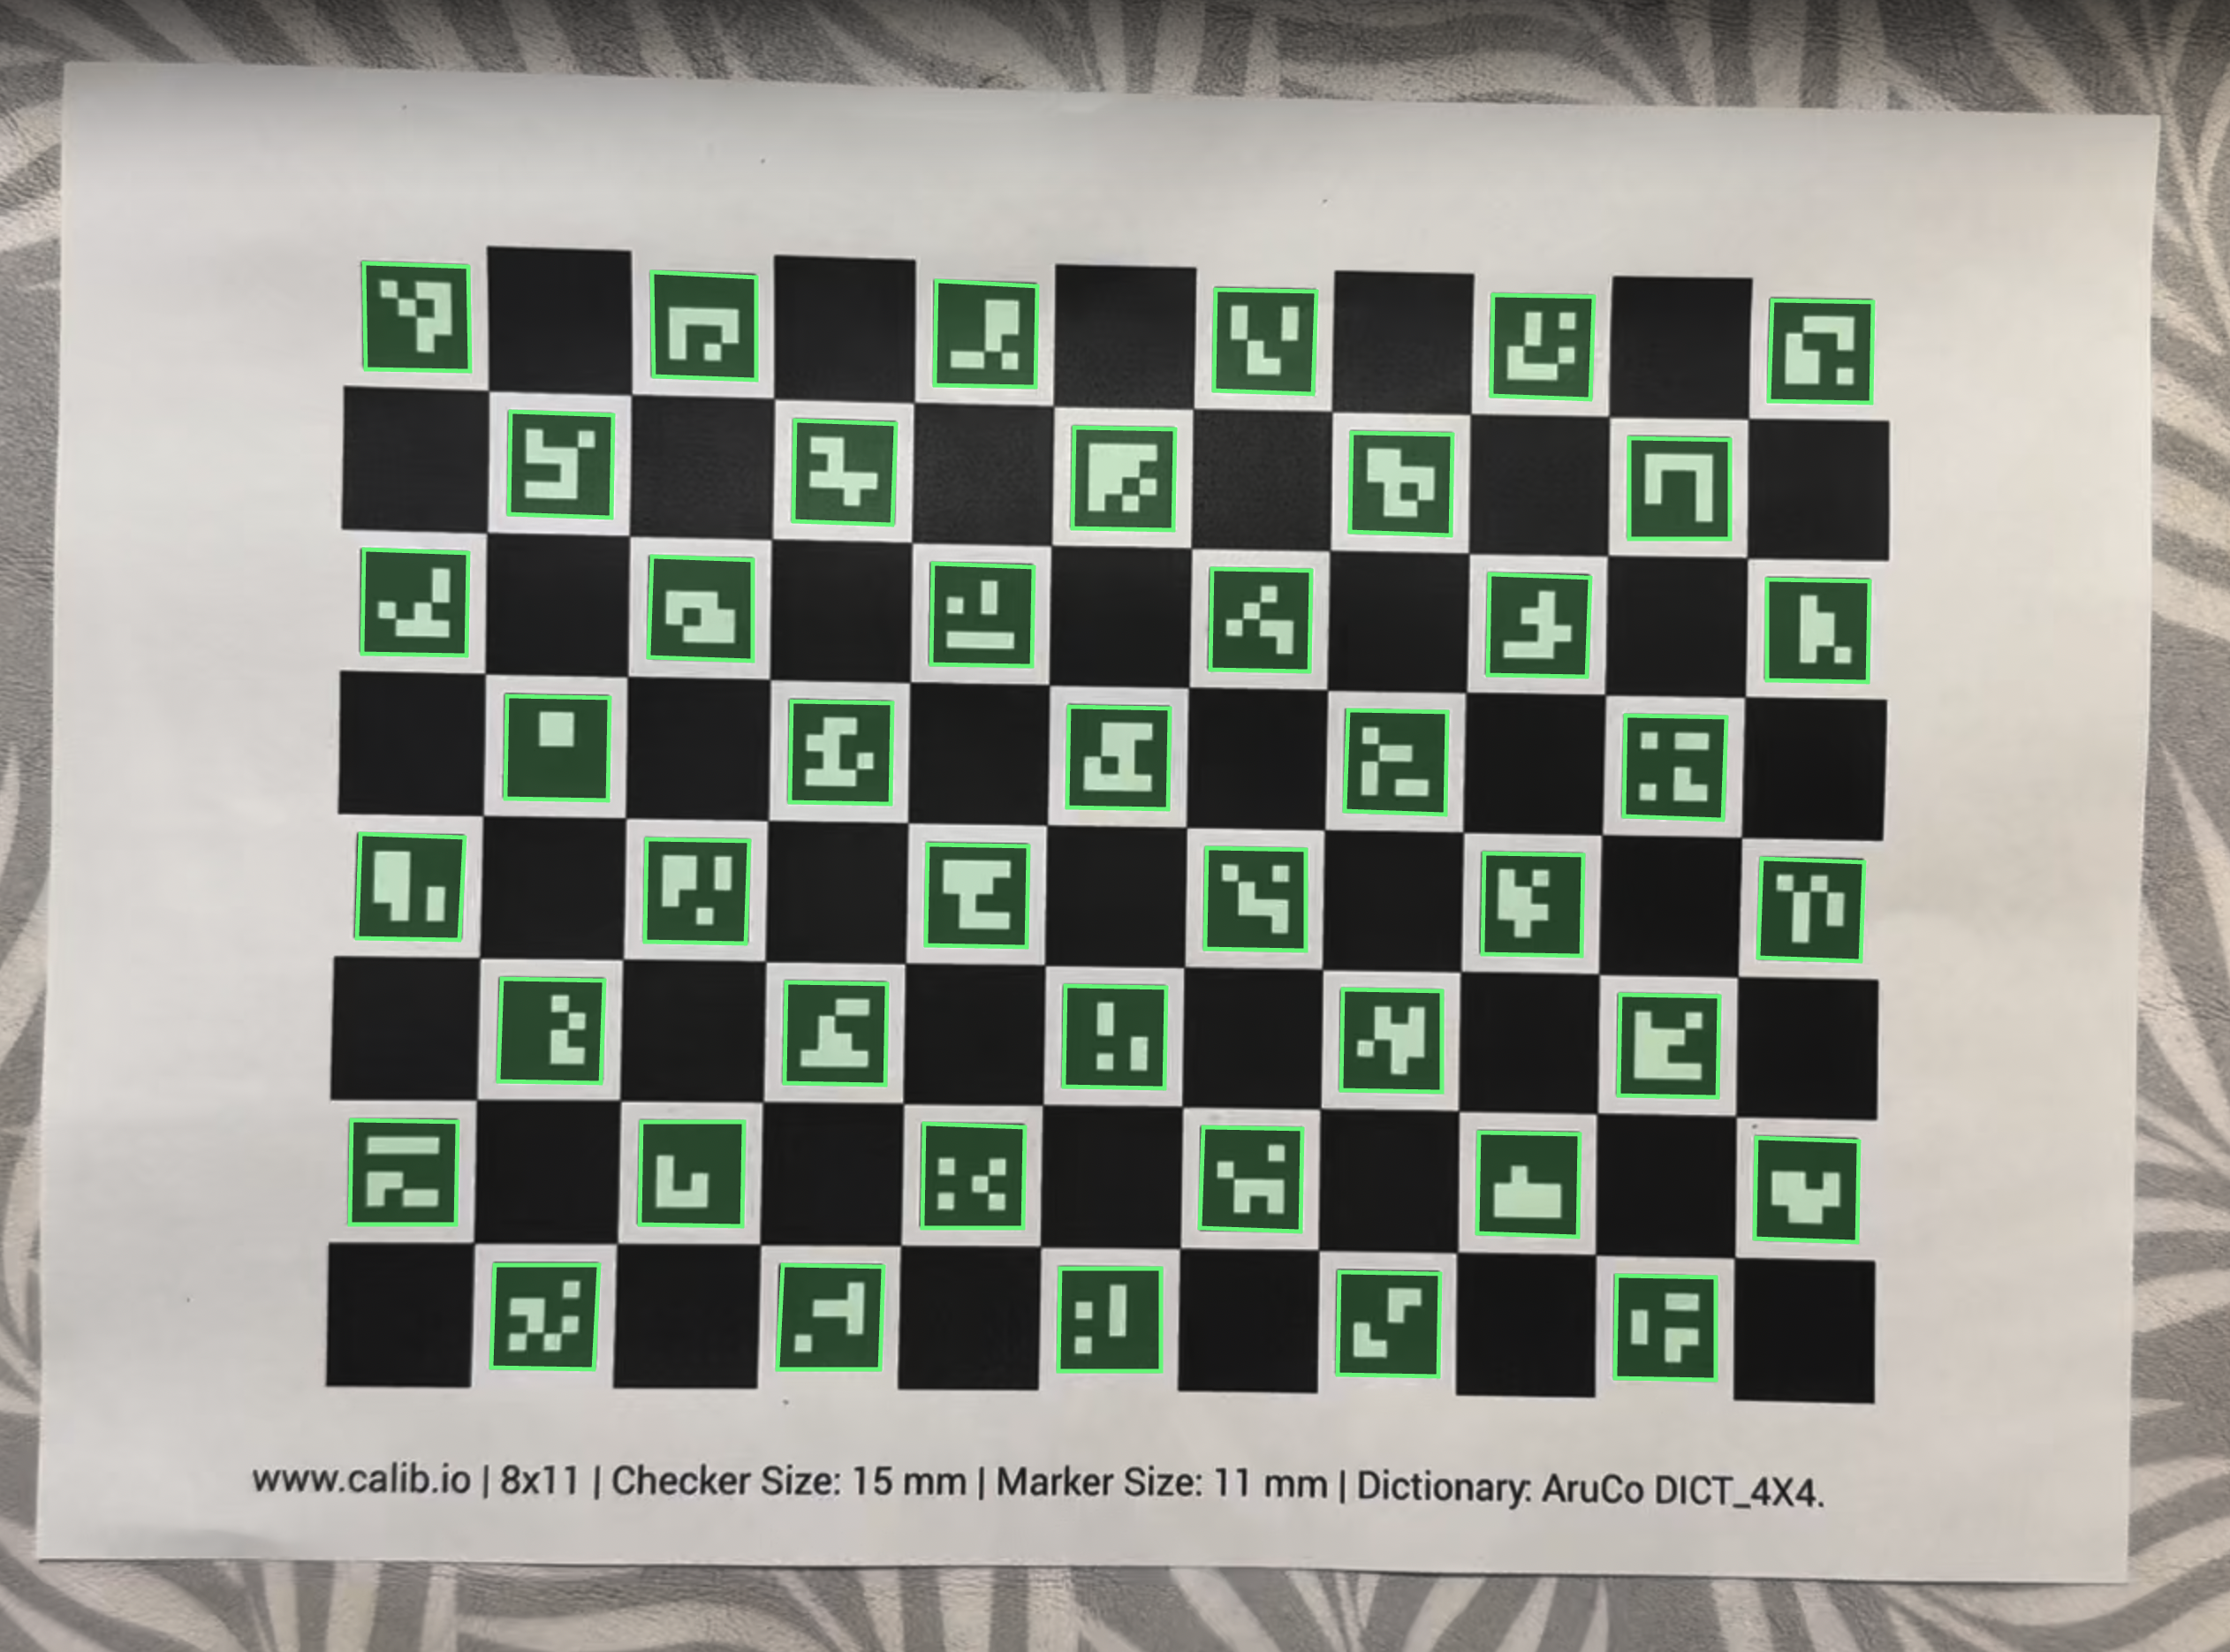
\includegraphics[width=0.80\textwidth]{Figures/cap_3/deteccion_charuco.png}
\caption{Detección del tablero ChArUco para estimación de relación milímetros por píxel.}
\label{fig:charuco-overlay}
\end{figure}

\subsection{Fase estática y segmentación del ejercicio}

En el ejercicio de finger tapping, los primeros segundos de muchas grabaciones corresponden a la mano en reposo sobre el tablero de calibración. Para excluir ese tramo del cálculo de métricas dinámicas se implementó \texttt{detect\_\allowbreak{}static\_\allowbreak{}calibration\_\allowbreak{}phase}, que calcula la desviación estándar móvil de la distancia pulgar--índice y marca como fase estática los intervalos en los que esa variabilidad permanece por debajo de 1{,}5~mm durante al menos 2~s. La función \texttt{slice\_\allowbreak{}dynamic\_\allowbreak{}after\_\allowbreak{}static} recorta la serie temporal a partir del final de esa fase. Opcionalmente, en la API, el parámetro \texttt{auto\_\allowbreak{}crop\_\allowbreak{}taps} acota además la ventana al intervalo entre el primero y el último pico de tapping detectado en la señal, con un margen temporal de 0{,}1~s a cada lado.

En la figura \ref{fig:static-phase} se observa una gráfica de la distancia pulgar--índice en función del tiempo, en la que se puede observar la fase estática y el inicio del segmento analizado para las métricas de tapping.

\vspace{0.6em}
\begin{center}
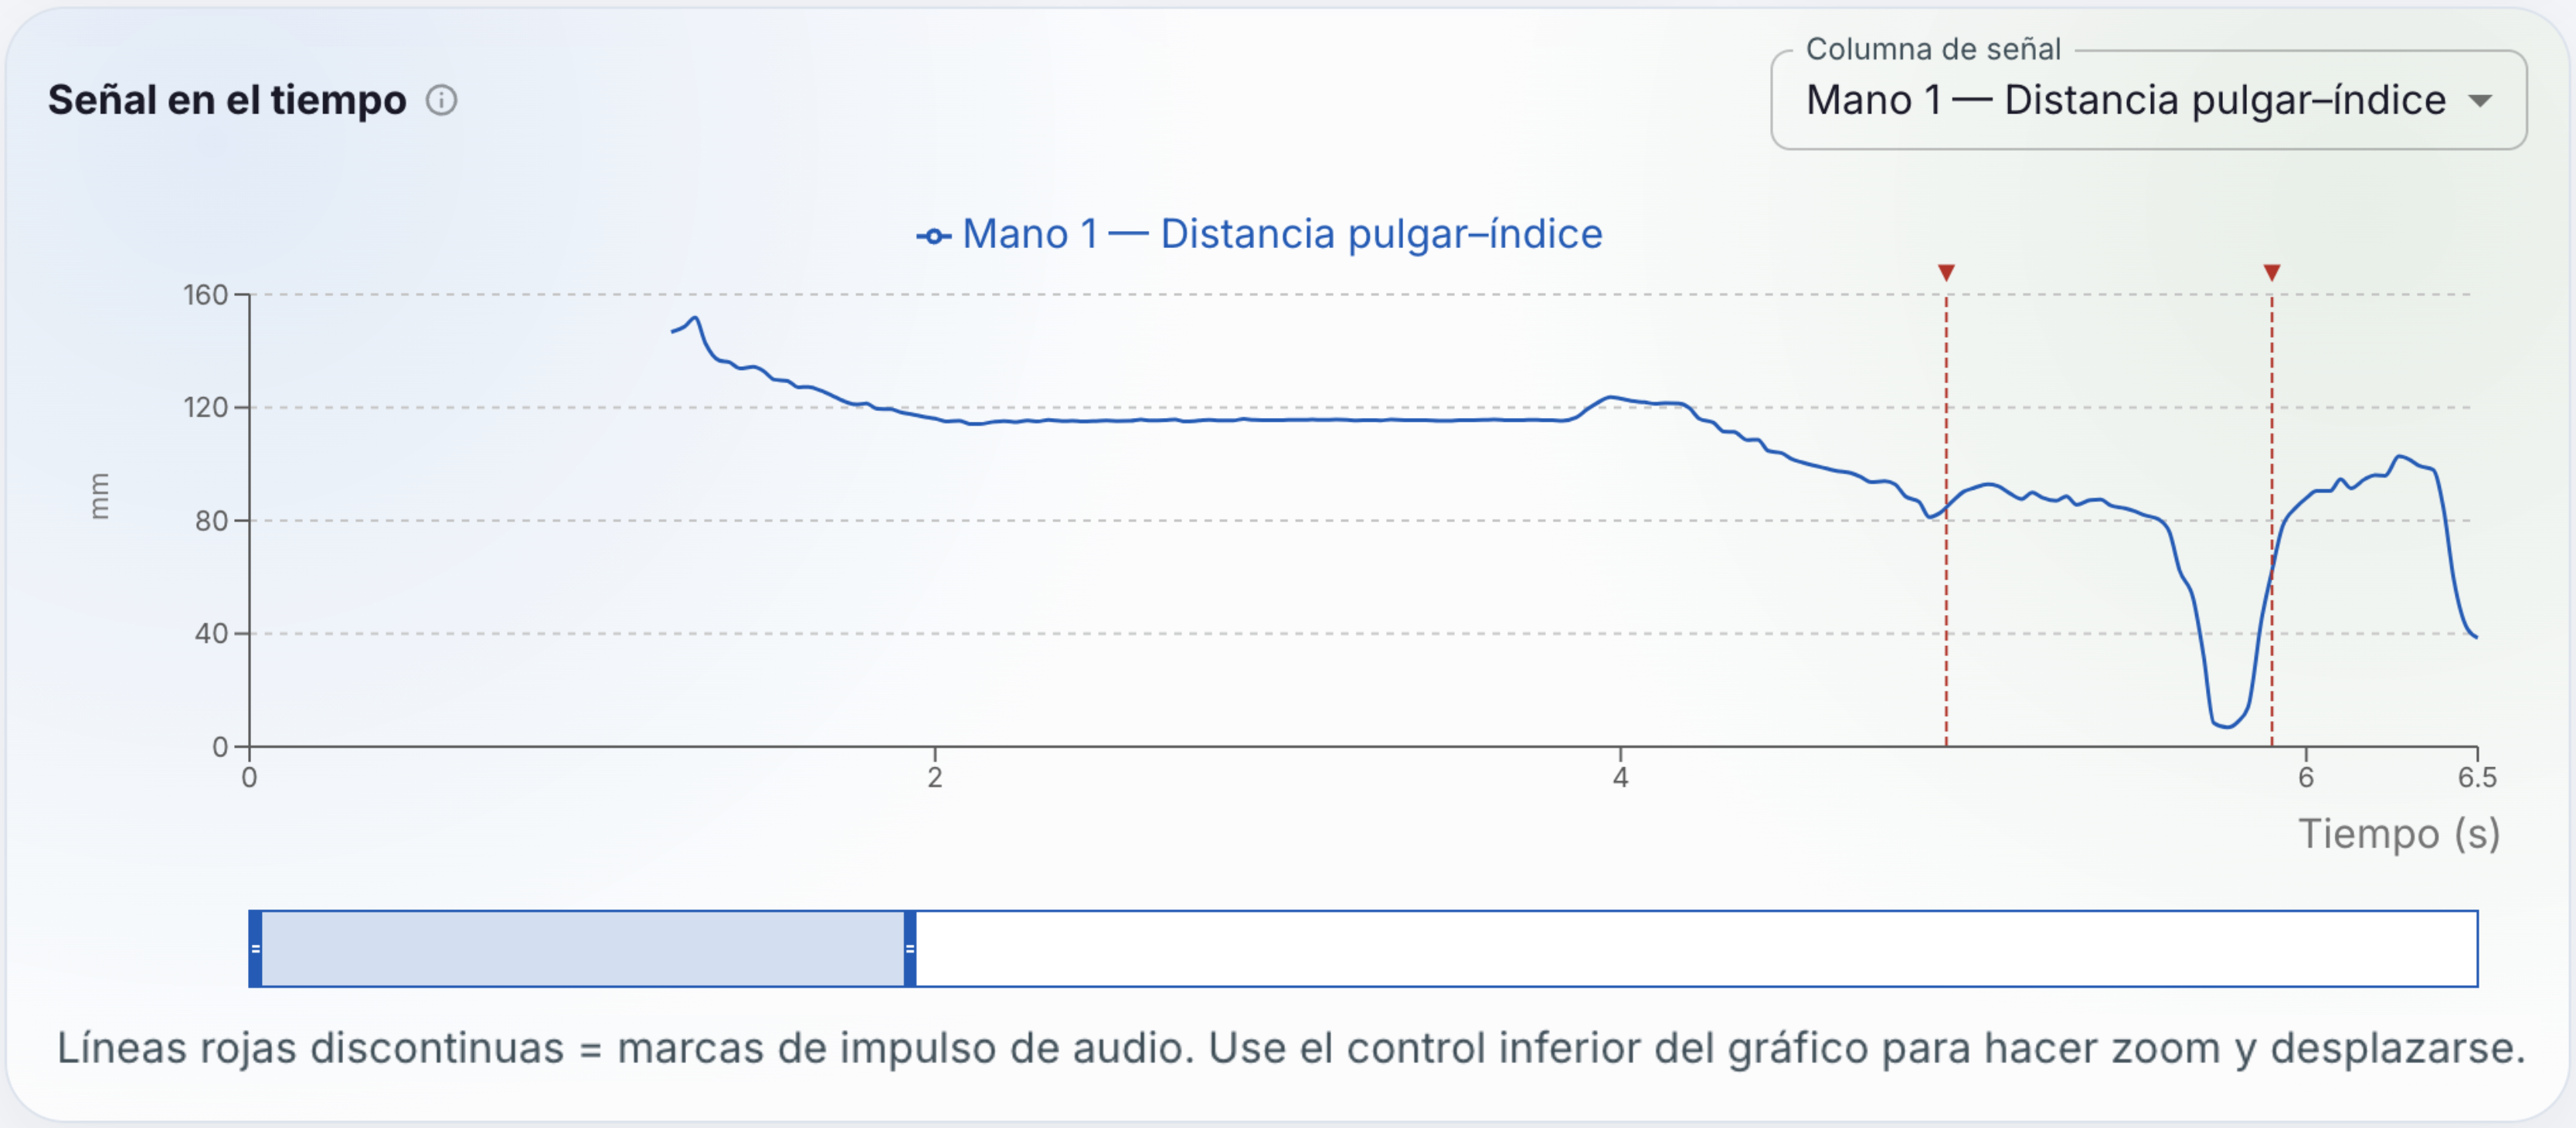
\includegraphics[width=0.90\textwidth]{Figures/cap_3/fase_estatica_dist_2.png}
\captionof{figure}{Fase estática de la distancia pulgar-índice en una sesión de finger tapping.}
\label{fig:static-phase}
\end{center}
\vspace{0.4em}

En la tabla \ref{tab:pipeline-etapas} se resumen las etapas del flujo de procesamiento, los datos que recibe y produce cada una, y los módulos del repositorio que implementan la transformación.

\begin{table}[H]
\centering
\caption{Etapas del pipeline de procesamiento de video y componentes asociados.}
\label{tab:pipeline-etapas}
{\setlength{\tabcolsep}{3.5pt}\footnotesize
\begin{tabular}{@{}>{\raggedright\arraybackslash}p{0.21\textwidth}>{\raggedright\arraybackslash}p{0.22\textwidth}>{\raggedright\arraybackslash}p{0.26\textwidth}>{\raggedright\arraybackslash}p{0.23\textwidth}@{}}
\toprule
\tabhead{Etapa} & \tabhead{Entrada} & \tabhead{Salida} & \tabhead{Módulo principal} \\
\midrule
Ingesta & Archivo de video. & Metadatos, audio mono, lista de impulsos. & \texttt{VideoLoader}, \texttt{AudioExtractor}. \\
Preprocesa-\\miento & Fotogramas BGR. & Fotogramas RGB redimensionados. & \texttt{FrameProcessor}. \\
Calibración & Muestra de fotogramas iniciales. & Factor mm/px y objeto \texttt{Calibration}. & \texttt{charuco}, \texttt{Calibration}. \\
Estimación de pose & Fotograma procesado. & \texttt{PoseResult} por cuadro. & \texttt{PoseEstimator}. \\
Seguimiento & Secuencia de \texttt{PoseResult}. & \texttt{DataFrame} por fotograma. & \texttt{KeypointTracker}. \\
Segmentación & Serie temporal completa. & Subserie para métricas (tapping). & \texttt{static\_phase}; recorte opcional. \\
Métricas & Serie de distancia pulgar--índice. & Lista de \texttt{MetricResult}. & \texttt{pipeline.metrics}. \\
Agregación y\\exportación & Tracking y métricas. & CSV, JSON, resumen de sesión. & \texttt{SessionAggregator} \\
\bottomrule
\end{tabular}}
\end{table}

Las etapas de ingesta, preprocesamiento y calibración corresponden al flujo documentado en esta sección. Las etapas de estimación de pose, seguimiento y segmentación se detallan en la sección~\ref{sec:arquitectura}.

%----------------------------------------------------------------------------------------

\section{Arquitectura de la solución analítica}
\label{sec:arquitectura}

Esta sección describe cómo se relaciona la inferencia con modelos ya presentados en el capítulo~\ref{Chapter2}, la construcción de series temporales a partir de landmarks y las magnitudes cuantitativas derivadas para cada sesión. Se omite el detalle de arquitecturas y pesos de terceros; el foco recae en la orquestación propia, el procesamiento de señales unidimensionales y la agregación orientada a la exploración clínica.

\subsection{Alcance del aprendizaje automático}

La arquitectura implementada se organizó como una cadena de módulos \texttt{Python} que orquestan inferencia con modelos preentrenados de visión, transforman las salidas en series temporales tabulares y calculan métricas en señales unidimensionales. En ese marco recayó el aporte principal del capítulo en materia de arquitectura: los contratos de datos entre etapas, el subsampleo temporal, la calibración, la agregación de sesión y el ajuste de parámetros de procesamiento de señal, umbrales de detección y reglas de segmentación documentadas en las subsecciones siguientes.

El alcance incluyó también un modelo de lenguaje de gran tamaño (LLM) como capa interpretativa sobre resultados ya cuantificados \citep{openai_api}, orientado a resúmenes por sesión y por evolución longitudinal. El servicio \texttt{/api/\allowbreak{}insights} consume exclusivamente el \texttt{summary.\allowbreak{}json} de sesiones finalizadas y no reenvía video ni coordenadas de landmarks al proveedor externo. Las instrucciones se versionaron en plantillas YAML \citep{yaml_spec} (\texttt{session\_\allowbreak{}summary.yaml} y \texttt{evolution\_\allowbreak{}summary.yaml}) con rol de sistema y plantilla de usuario separados, de modo que el equipo pudiera iterar el texto sin modificar el código del enrutador.

Durante la implementación se evaluaron distintas variantes de prompt para acotar tono y extensión de la respuesta generada. Se fijó temperatura baja, límites de tokens de salida, secciones con encabezados predefinidos y prohibición explícita de formular diagnósticos, con recordatorio de que la interpretación final debe ser validada por el personal médico. Las variables interpoladas en cada solicitud se limitaron a metadatos de sesión, indicadores de calidad de la captura y tablas de métricas agregadas, sin nombres ni grabaciones del paciente, en línea con la política de manejo de datos del trabajo. El acceso al endpoint exige autenticación y verificación de que la sesión pertenece al profesional solicitante antes de invocar al modelo.

\subsection{Criterios de diseño y configuración}

La configuración global se centralizó en la clase \texttt{Settings}, que se carga con prefijo de variables de entorno \texttt{DAGO\_} y valores por defecto versionados en el repositorio. De ese modo se evitó codificar rutas, umbrales de audio o geometría del tablero ChArUco dentro de la lógica. El tipo de ejercicio clínico (\texttt{finger\_tapping}, \texttt{hand\_tremor}, \texttt{nose\_finger}, \texttt{open\_close\_hands}) se propagó a lo largo del pipeline para etiquetar métricas y seleccionar el modelo de pose adecuado.

Se adoptó además una política de clasificación de datos en tres niveles en el repositorio: material de muestra anonimizado apto para integración continua, grabaciones reales de pacientes excluidas del control de versiones y directorios de salida de análisis ignorados por el sistema de seguimiento de cambios. Esa separación se mantuvo coherente con los requerimientos éticos de la planificación inicial y condicionó que las pruebas automatizadas y los ejemplos de documentación apuntaran únicamente al nivel público, mientras las sesiones clínicas reales se procesaron en entornos locales o en la nube con almacenamiento privado.

\subsection{Contrato de datos entre etapas}

Para mantener la trazabilidad entre módulos se definieron esquemas de datos inmutables en cada frontera. \texttt{VideoMeta} y \texttt{FrameData} describen el origen temporal de cada fotograma; \texttt{AudioData} e \texttt{ImpulseEvent} encapsulan el audio y los pulsos detectados; \texttt{ProcessedFrame} añade las transformaciones de imagen; \texttt{Pose\allowbreak{}Result} agrupa las detecciones de mano y cuerpo por cuadro; y \texttt{Metric\allowbreak{}Result} estandariza la salida de cada algoritmo de métrica con nombre, unidad, validez y metadatos opcionales. El resumen final de sesión (\texttt{Session\allowbreak{}Summary}) consolida métricas, retardos, parámetros de calibración, metrónomo y versión del pipeline en un único documento JSON serializable, apto para persistencia relacional y para los prompts del modelo de lenguaje.

Ese contrato permite sustituir o extender un módulo sin alterar los demás siempre que respete las interfaces acordadas. Por ejemplo, un futuro estimador de pose alternativo podría devolver el mismo \texttt{PoseResult} sin modificar el seguimiento ni las métricas aguas abajo.

\subsection{Orquestación de la inferencia}

El sistema se diseñó para no depender de un único modelo monolítico. La función \texttt{pose\_model\_for\_exercise} selecciona el landmarker de \texttt{MediaPipe} según el tipo de ejercicio para extraer las señales de alta frecuencia: modo \texttt{HANDS} para \texttt{finger\_tapping}, \texttt{hand\_tremor} y \texttt{open\_close\_hands}, y modo \texttt{HOLISTIC} para \texttt{nose\_finger}. La clase \texttt{PoseEstimator} instancia el modelo correspondiente mediante la API de tareas, con archivos \texttt{.task} en caché local. En paralelo y de forma específica para los fotogramas iniciales, el modelo MeTRAbs se orquesta para resolver la profundidad métrica y establecer el factor de escala global de la sesión.

La coordenada de profundidad (\texttt{z}) de \texttt{MediaPipe} se registró en los esquemas internos, pero las medidas métricas se calcularon en dos dimensiones con la calibración inicial. En modo \texttt{HANDS} se conservó una mano dominante por fotograma; en \texttt{HOLISTIC}, también hombros, codos y muñecas para visualización.

En la figura \ref{fig:pipeline-dago} se resume el flujo desde el video crudo hasta reportes y consulta, con estimación de pose, procesamiento analítico, persistencia y acceso por API y web (sección \ref{sec:integracion}).

\begin{figure}[H]
\centering
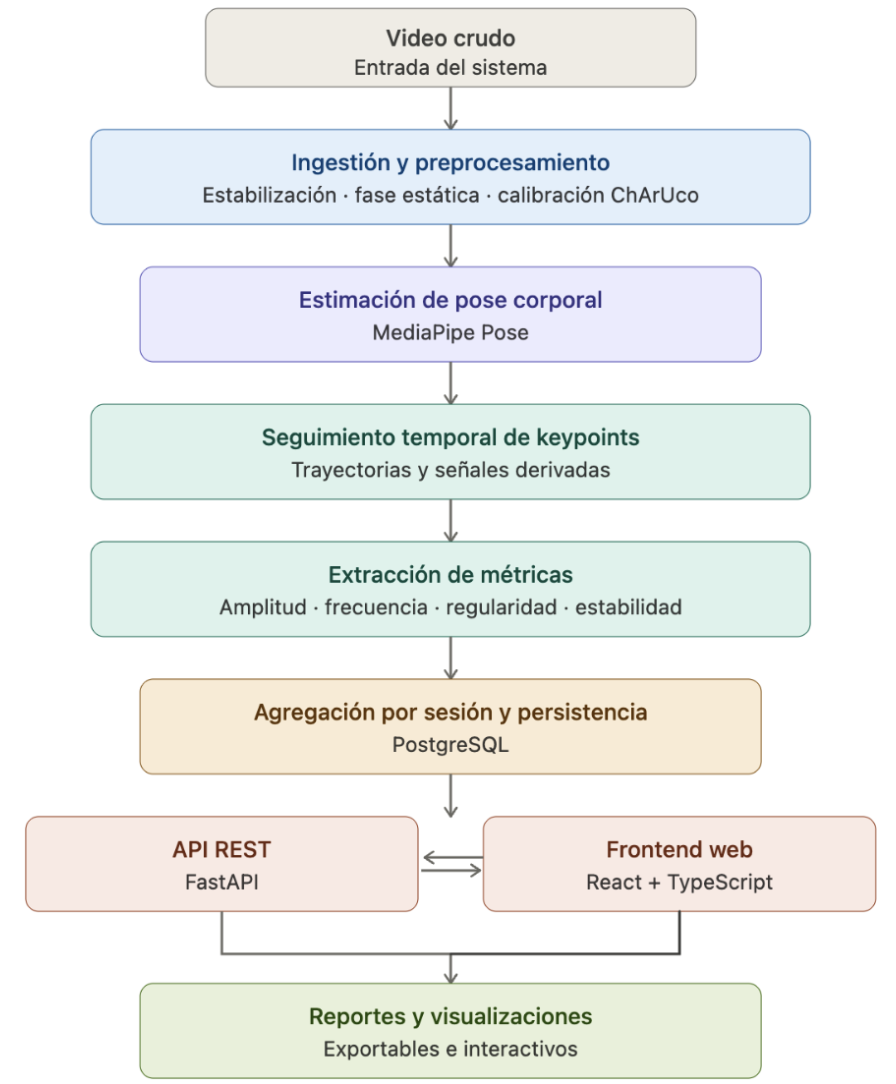
\includegraphics[width=0.72\textwidth]{Figures/cap_3/diagrama_flujo_dago.png}
\caption{Flujo funcional del sistema desde la entrada de video hasta reportes y visualizaciones.}
\label{fig:pipeline-dago}
\end{figure}

\subsection{Seguimiento temporal y señales derivadas}

\texttt{KeypointTracker} acumula, por cada fotograma analizado, un registro tabular común con índice temporal, coordenadas normalizadas de los 21 puntos de la mano dominante, distancias derivadas en milímetros cuando existe calibración y, en modo holístico, posiciones de nariz, hombros, codos y muñecas junto con los ángulos de abducción de brazo izquierdo y derecho (\texttt{pose\_left\_arm\_angle}, \texttt{pose\_right\_arm\_angle}). Las detecciones ausentes se registran como valores faltantes y se rellenan hacia adelante hasta un máximo de cinco fotogramas consecutivos para atenuar oclusiones breves. Esa capa de seguimiento es compartida por los cuatro tipos de ejercicio, pero la señal que alimenta las métricas clínicas se elige en función del movimiento evaluado.

En \texttt{finger\_tapping} la señal operativa principal es la distancia pulgar--índice \texttt{hand0\_\allowbreak{}thumb\_\allowbreak{}index\_\allowbreak{}dist}. Con factor de escala $s$ milímetros por píxel y coordenadas normalizadas de pulgar e índice $\mathbf{p}_t$ y $\mathbf{q}_t$ en un fotograma de ancho $W$ y alto $H$ píxeles, se define la distancia $d_t$ mediante la ecuación \ref{eq:thumb-index-dist}:
\begin{equation}
d_t = s \,\sqrt{W^2(p_{t,x}-q_{t,x})^2 + H^2(p_{t,y}-q_{t,y})^2}\,.
\label{eq:thumb-index-dist}
\end{equation}
\begin{sloppypar}
En \texttt{finger\_tapping}, $d_t$ sustentó los biomarcadores de tapping y la sincronía con el metrónomo. En \texttt{hand\_tremor}, las trayectorias de los dedos índice, medio y anular de cada mano (asignadas a izquierda y derecha según la posición en imagen) alimentaron el cuantificador \texttt{TremorQuantifier}, que estimó amplitud y frecuencia del temblor postural por extremidad. En \texttt{open\_close\_hands}, la apertura de cada mano se expresó mediante las columnas \texttt{left\_\allowbreak{}hand\_\allowbreak{}openness\_\allowbreak{}mm} y \texttt{right\_\allowbreak{}hand\_\allowbreak{}openness\_\allowbreak{}mm}, obtenidas al reasignar los slots \texttt{hand0}/\texttt{hand1} de MediaPipe a la anatomía del paciente.
\end{sloppypar}

En \texttt{nose\_finger} se normalizó la distancia yema del índice--nariz por el ancho de hombros y se obtuvieron \texttt{left\_\allowbreak{}finger\_\allowbreak{}nose\_\allowbreak{}norm} y \texttt{right\_\allowbreak{}finger\_\allowbreak{}nose\_\allowbreak{}norm}. Los mínimos locales de esas series delimitaron contactos con la nariz; se validaron la postura inicial en cruz, la extensión del brazo contrario y el retorno al alcance. Como métricas secundarias se registraron la variabilidad del ángulo de abducción de cada brazo y la estabilidad postural del tronco mediante un proxy hombro--cadera.

\subsection{Métricas de movimiento implementadas}

\begin{sloppypar}
El módulo de métricas seleccionó, según el tipo de ejercicio, la señal temporal y el conjunto de algoritmos aplicables. En \texttt{finger\_tapping}, las funciones \texttt{oscillation\_\allowbreak{}amplitude}, \texttt{tremor\_\allowbreak{}frequency} y \texttt{movement\_\allowbreak{}regularity} operaron sobre $\{d_t\}$ cuando hubo al menos cuatro muestras válidas; la frecuencia dominante se estimó por transformada rápida de Fourier en la banda definida en la ecuación \ref{eq:tremor-band}:
\end{sloppypar}
\begin{equation}
f \in [1{,}0,\, 12{,}0]\ \text{Hz},
\label{eq:tremor-band}
\end{equation}
coherente con el rango de interés clínico para temblor y oscilaciones de extremidad superior \citep{pecoraro2025computer}, para lo cual se empleó la tasa efectiva tras el subsampleo ($f_s = \mathrm{fps}_{\mathrm{video}} / \mathrm{step}$).

\begin{sloppypar}
En \texttt{finger\_tapping}, tras recortar la fase estática y, de manera opcional, la ventana entre el primero y el último tap, se aplicaron sobre $\{d_t\}$ los biomarcadores de \texttt{compute\_\allowbreak{}finger\_\allowbreak{}tapping\_\allowbreak{}metrics}: tasa de taps, intervalo intertap medio y su coeficiente de variación, decremento de amplitud entre picos, índice de fatiga, velocidades medias de apertura y cierre, y el promedio del ángulo en la muñeca (\texttt{thumb\_\allowbreak{}index\_\allowbreak{}wrist\_\allowbreak{}angle\_\allowbreak{}mean}). La detección de picos usó \texttt{scipy.\allowbreak{}signal.\allowbreak{}find\_\allowbreak{}peaks} con prominencia proporcional al rango de la señal \citep{sibley2021video,acevedo2025visionmd}. \texttt{SessionAggregator} calculó además retardos entre impulsos del metrónomo y mínimos locales de $d_t$ dentro de $\pm 0{,}35$~s, exportados en \texttt{delays.csv} y en el resumen como \texttt{movement\_\allowbreak{}delays} (no como magnitud escalar en \texttt{metrics.csv}).

En \texttt{hand\_tremor}, \texttt{TremorQuantifier} aplicó un filtro pasabanda Butterworth entre 2 y 10~Hz sobre la trayectoria promedio de los tres dedos y estimó, por mano, la amplitud pico a pico (\texttt{tremor\_\allowbreak{}amplitude\_\allowbreak{}left/\allowbreak{}right}) y la frecuencia principal por método de Welch (\texttt{tremor\_\allowbreak{}frequency\_\allowbreak{}left/\allowbreak{}right}). No se calcularon biomarcadores de tapping, regularidad de movimiento ni retardos con metrónomo.

En \texttt{nose\_finger}, \texttt{compute\_\allowbreak{}nose\_\allowbreak{}finger\_\allowbreak{}metrics} cuantificó repeticiones válidas, contactos por mano, ritmo alternado, sincronía con el metrónomo, amplitud de alcance normalizada, velocidades de aproximación y retorno, asimetrías bilaterales, suavidad del gesto y oscilación durante el alcance. Como métricas secundarias se estimaron \texttt{postural\_\allowbreak{}stability} y \texttt{arm\_\allowbreak{}angle\_\allowbreak{}variability\_\allowbreak{}left/\allowbreak{}right} a partir del desplazamiento del centro de masa definido por hombros y caderas y del rango del ángulo de abducción de cada brazo.

En \texttt{open\_close\_hands}, \texttt{compute\_\allowbreak{}open\_\allowbreak{}close\_\allowbreak{}hands\_\allowbreak{}metrics} procesó las series bilaterales de apertura para obtener tasas de cierre por mano, intervalos entre cierres, decremento y fatiga de amplitud, velocidades en picos y valles, y asimetrías de amplitud, ritmo, velocidad y alineación con el metrónomo cuando el audio estaba disponible.
\end{sloppypar}

Cada magnitud se encapsuló en un \texttt{MetricResult} con unidad, validez y nota cuando los datos fueron insuficientes. En el listado siguiente se resume el catálogo por tipo de ejercicio.\label{sec:metricas-implementadas}

\begin{sloppypar}
\begin{itemize}
    \item Tapping de dedos:
    \begin{itemize}
        \item Amplitud de oscilación (\texttt{oscillation\_\allowbreak{}amplitude}, mm): rango pico a pico de $d_t$.
        \item Frecuencia de temblor (\texttt{tremor\_\allowbreak{}frequency}, Hz): pico espectral sobre $d_t$, banda definida según la ecuación \ref{eq:tremor-band}.
        \item Regularidad del movimiento (\texttt{movement\_\allowbreak{}regularity}, adim.): variabilidad y entropía muestral de $d_t$.
        \item Tasa de taps (\texttt{tap\_rate}, 1/s): ritmo de taps asociado a bradicinesia.
        \item Intervalo intertap medio (\texttt{iti\_mean}, s): tiempo medio entre taps consecutivos.
        \item Coeficiente de variación del ITI (\texttt{iti\_cv}, adim.): consistencia del ritmo de tapping.
        \item Decremento de amplitud (\texttt{amplitude\_\allowbreak{}decrement}, mm/s): pendiente de amplitud entre picos sucesivos.
        \item Índice de fatiga (\texttt{fatigue\_\allowbreak{}index}, adim.): amplitud final respecto de la amplitud inicial en la ventana dinámica.
        \item Velocidad de apertura en picos (\texttt{peak\_\allowbreak{}opening\_\allowbreak{}velocity}, mm/s): velocidad media al abrir los dedos en los picos de $d_t$.
        \item Velocidad de cierre en valles (\texttt{peak\_\allowbreak{}closing\_\allowbreak{}velocity}, mm/s): velocidad media al cerrar los dedos en los valles.
        \item Ángulo medio en muñeca (\texttt{thumb\_\allowbreak{}index\_\allowbreak{}wrist\_\allowbreak{}angle\_\allowbreak{}mean}, $^{\circ}$): apertura media pulgar--índice en la muñeca.
        \item Retardos audio--movimiento (\texttt{movement\_\allowbreak{}delays}, s): desfase por impulso entre el metrónomo y el mínimo local de $d_t$ en $\pm 0{,}35$~s (\texttt{delays.csv}); no se agregó como escalar único en \texttt{metrics.csv}.
    \end{itemize}

    \item Temblor de mano:
    \begin{itemize}
        \item Amplitud de temblor (\texttt{tremor\_\allowbreak{}amplitude\_\allowbreak{}left/\allowbreak{}right}, mm): rango pico a pico filtrado de la trayectoria promedio índice--medio--anular.
        \item Frecuencia de temblor (\texttt{tremor\_\allowbreak{}frequency\_\allowbreak{}left/\allowbreak{}right}, Hz): frecuencia principal por Welch en banda 2--10~Hz.
    \end{itemize}

    \item Prueba nariz--dedo:
    \begin{itemize}
        \item Repeticiones completadas (\texttt{repetitions\_\allowbreak{}completed}, cont.): toques válidos con brazo contrario extendido y retorno a la postura en cruz.
        \item Tasa de éxito (\texttt{touch\_\allowbreak{}success\_\allowbreak{}rate}, adim.): cociente entre repeticiones válidas y aproximaciones detectadas.
        \item Conteo de contactos (\texttt{touch\_\allowbreak{}count\_\allowbreak{}left/\allowbreak{}right}, \texttt{failed\_\allowbreak{}touches}, cont.): aproximaciones por mano y fallos de protocolo.
        \item Ritmo de contactos (\texttt{touch\_rate}, 1/s; \texttt{iti\_mean}, s; \texttt{iti\_cv}, adim.): cadencia alternada entre manos.
        \item Sincronía con metrónomo (\texttt{on\_\allowbreak{}beat\_\allowbreak{}ratio}, adim.; \texttt{timing\_\allowbreak{}error\_\allowbreak{}mean}, \texttt{timing\_\allowbreak{}error\_\allowbreak{}abs\_\allowbreak{}mean}, s; \texttt{timing\_\allowbreak{}cv}, adim.): desfase respecto de los impulsos de audio.
        \item Amplitud de alcance (\texttt{reach\_\allowbreak{}amplitude\_\allowbreak{}left/\allowbreak{}right}, adim.): rango normalizado (referencia extendida menos contacto, / hombros).
        \item Velocidades de aproximación y retorno (\texttt{approach\_\allowbreak{}velocity\_\allowbreak{}left/\allowbreak{}right}, \texttt{return\_\allowbreak{}velocity\_\allowbreak{}left/\allowbreak{}right}, adim./s): picos de velocidad hacia la nariz y de vuelta.
        \item Asimetrías (\texttt{amplitude\_\allowbreak{}asymmetry}, \texttt{velocity\_\allowbreak{}asymmetry}, \texttt{count\_\allowbreak{}asymmetry}, \texttt{rhythm\_\allowbreak{}asymmetry}, adim.): diferencias bilaterales de alcance, velocidad, conteo y ritmo.
        \item Suavidad del gesto (\texttt{movement\_\allowbreak{}smoothness\_\allowbreak{}left/\allowbreak{}right}, adim.): regularidad de la trayectoria índice--nariz por mano.
        \item Oscilación en el alcance (\texttt{tremor\_\allowbreak{}frequency\_\allowbreak{}left/\allowbreak{}right}, Hz): componente espectral baja del dedo índice durante el movimiento.
        \item Estabilidad postural (\texttt{postural\_\allowbreak{}stability}, adim./fotograma): balanceo del tronco, estimado como proxy hombro--cadera (métrica secundaria).
        \item Variabilidad del ángulo de abducción (\texttt{arm\_\allowbreak{}angle\_\allowbreak{}variability\_\allowbreak{}left/\allowbreak{}right}, $^{\circ}$): rango pico a pico del ángulo de brazo (métrica secundaria; la media figura en los metadatos de la métrica).
    \end{itemize}

    \item Apertura y cierre de manos:
    \begin{itemize}
        \item Tasa de ciclos (\texttt{cycle\_\allowbreak{}rate\_\allowbreak{}left/\allowbreak{}right}, 1/s): eventos de cierre por segundo en cada mano.
        \item Amplitud media de apertura (\texttt{mean\_\allowbreak{}openness\_\allowbreak{}amplitude\_\allowbreak{}left/\allowbreak{}right}, mm): apertura media en los cierres detectados.
        \item Intervalos entre cierres (\texttt{iti\_\allowbreak{}mean\_\allowbreak{}close\_\allowbreak{}left/\allowbreak{}right}, s; \texttt{iti\_\allowbreak{}cv\_\allowbreak{}close\_\allowbreak{}left/\allowbreak{}right}, adim.): ritmo y consistencia por mano.
        \item Decremento de amplitud (\texttt{amplitude\_\allowbreak{}decrement\_\allowbreak{}left/\allowbreak{}right}, mm/s): pendiente de amplitud en cierres sucesivos.
        \item Índice de fatiga (\texttt{fatigue\_\allowbreak{}index\_\allowbreak{}left/\allowbreak{}right}, adim.): cociente entre amplitud del último y primer tercio de cierres.
        \item Velocidad de apertura en picos (\texttt{peak\_\allowbreak{}opening\_\allowbreak{}velocity\_\allowbreak{}left/\allowbreak{}right}, mm/s): velocidad media al abrir cada mano.
        \item Velocidad de cierre en valles (\texttt{peak\_\allowbreak{}closing\_\allowbreak{}velocity\_\allowbreak{}left/\allowbreak{}right}, mm/s): velocidad media al cerrar cada mano.
        \item Asimetrías bilaterales (\texttt{amplitude\_\allowbreak{}asymmetry}, \texttt{rhythm\_\allowbreak{}asymmetry\_\allowbreak{}iti}, \texttt{velocity\_\allowbreak{}asymmetry\_\allowbreak{}open/\allowbreak{}close}, \texttt{fatigue\_\allowbreak{}asymmetry}, adim.): comparación relativa entre manos.
        \item Alineación con metrónomo (\texttt{inter\_\allowbreak{}hand\_\allowbreak{}timing\_\allowbreak{}lag}, s; \texttt{mean\_\allowbreak{}close/\allowbreak{}open\_\allowbreak{}delay\_\allowbreak{}left/\allowbreak{}right}, s): retardos por mano y fase cuando hubo audio disponible.
    \end{itemize}
\end{itemize}
\end{sloppypar}

En la figura \ref{fig:timeseries-metricas} se ilustra, a modo de ejemplo para \texttt{finger\_tapping}, la serie $d_t$ con picos de tapping y las detecciones de los pulsos del metrónomo marcados con líneas verticales rojas.

\begin{figure}[htbp]
\centering
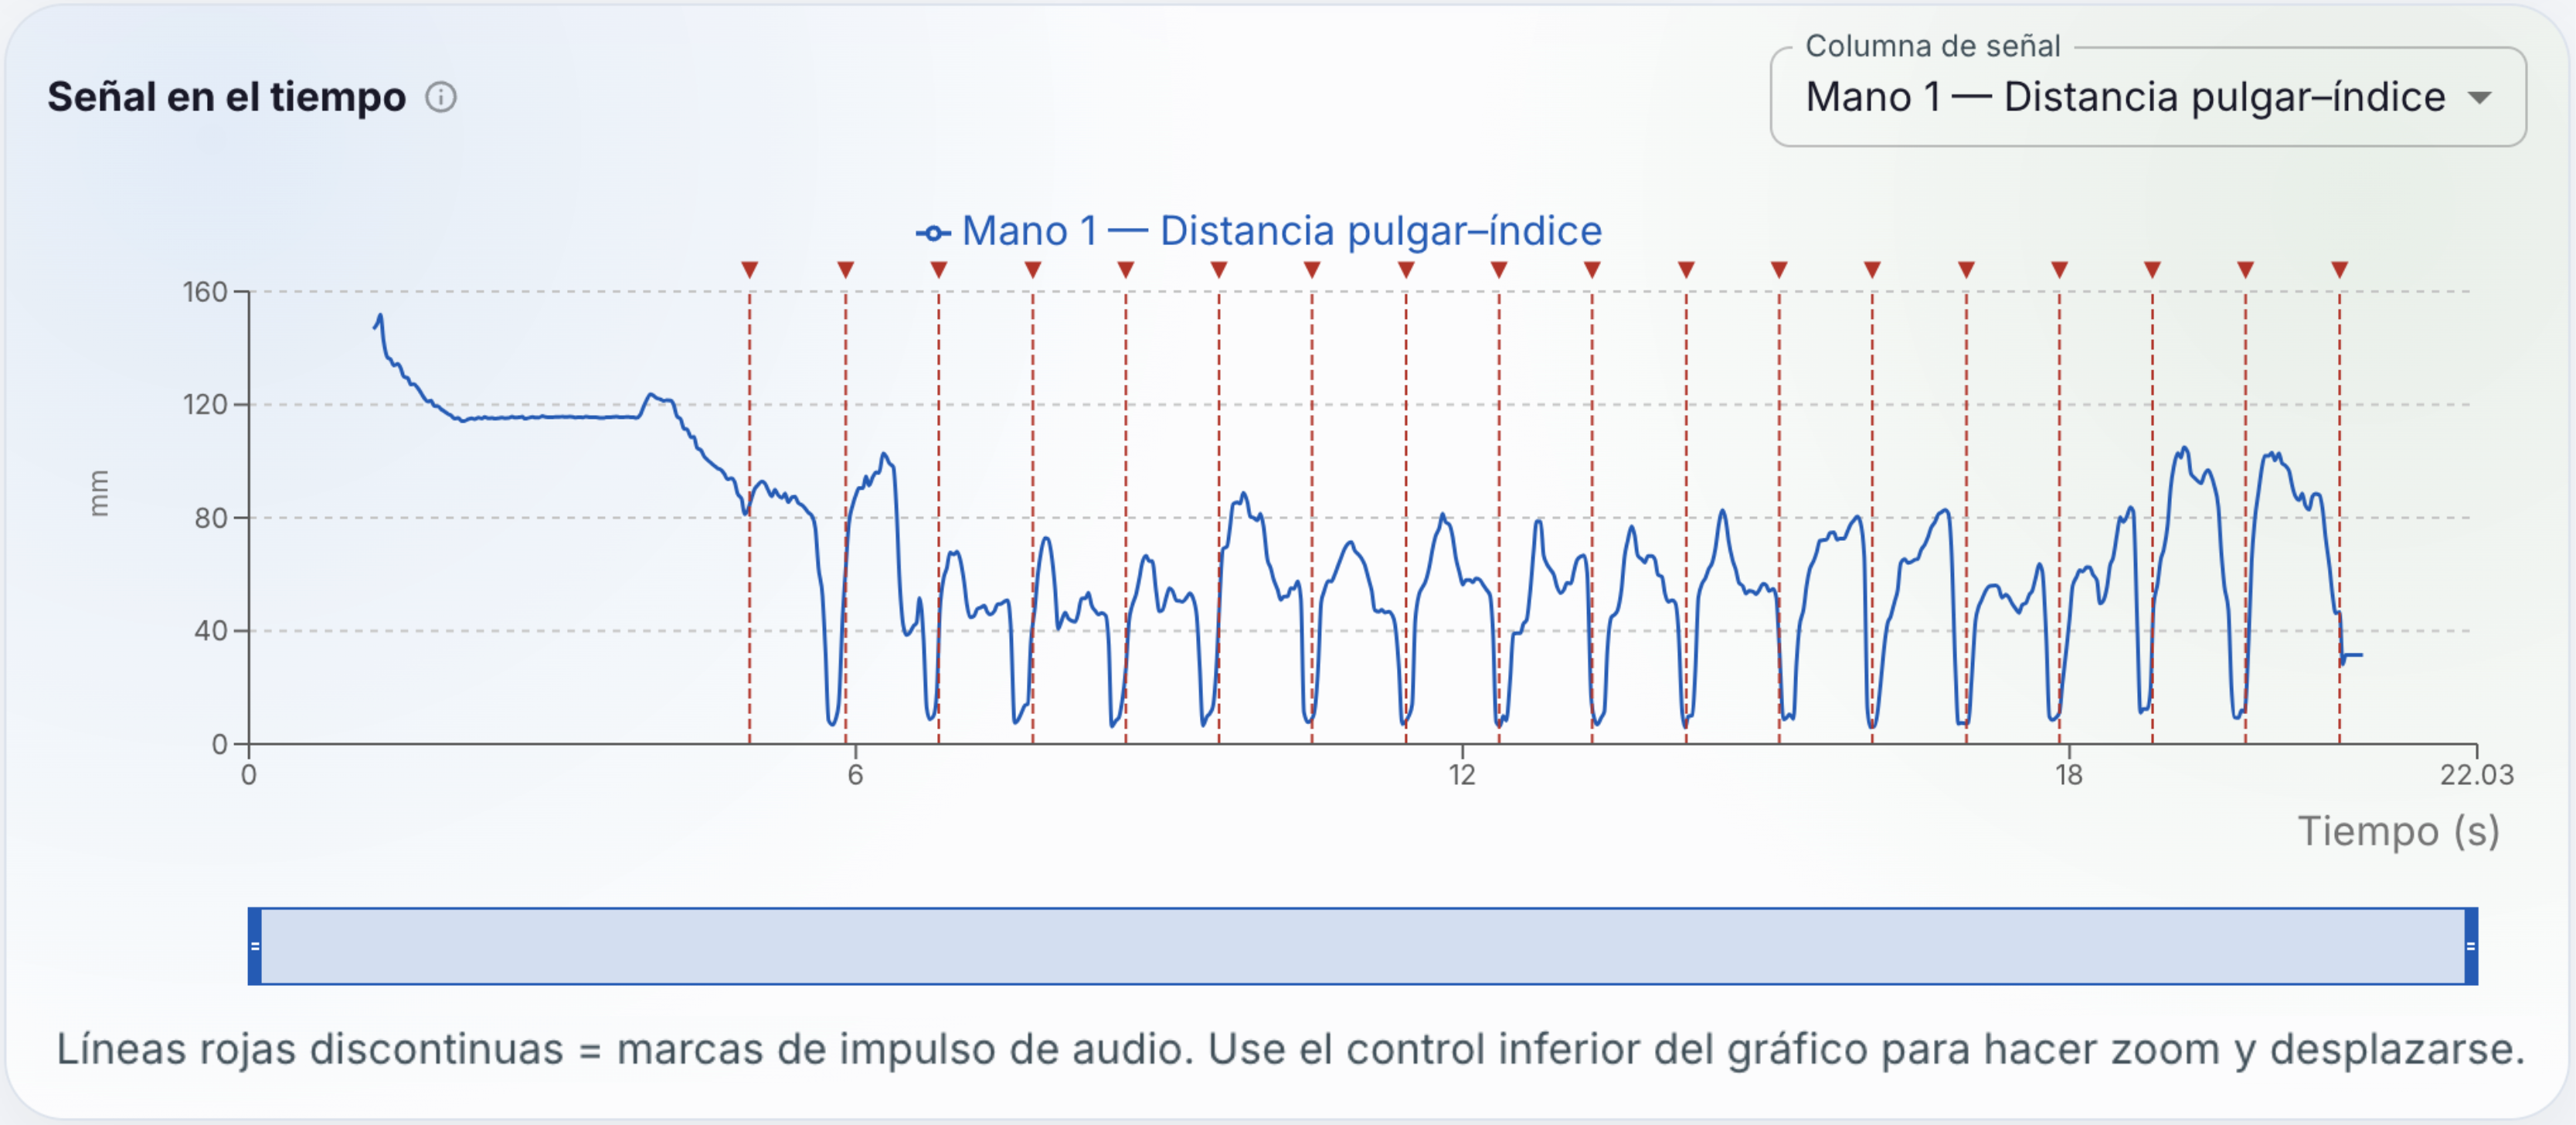
\includegraphics[width=0.95\textwidth]{Figures/cap_3/sesion_completa_dist_2.png}
\caption{Serie temporal de la distancia pulgar--índice durante una sesión completa.}
\label{fig:timeseries-metricas}
\end{figure}

\begin{sloppypar}
En la ejecución por línea de comandos se generan además gráficos \texttt{timeseries.png}, \texttt{metrics\_summary.png} y \texttt{detection\_overview.png} cuando la opción de guardado de figuras está activa. El worker de la API omite esos gráficos para reducir tiempo y uso de memoria en el contenedor y delega la visualización interactiva al frontend.
\end{sloppypar}

\subsection{Agregación, exportación y trazabilidad}

\texttt{SessionAggregator} recibe el \texttt{DataFrame} completo de seguimiento (incluida la fase estática cuando corresponde), la lista de métricas calculadas, los impulsos de audio y los metadatos de calibración. Produce un resumen con identificador de video, tipo de ejercicio, tasa de fotogramas nominal, conteo de fotogramas analizados, tabla de métricas y colección de retardos audio--movimiento. Los componentes \texttt{CsvWriter} y \texttt{JsonWriter} materializan ese contenido en disco con convenciones de nombres de columna estables, de modo que las pruebas de integración puedan verificar la existencia y el esquema de \texttt{tracking.csv}, \texttt{metrics.csv} y \texttt{summary.json} tras una ejecución de prueba del comando de sesión.

La coherencia entre definiciones matemáticas en código y descripción en la memoria se verificó en el capítulo~\ref{Chapter4} mediante pruebas unitarias sobre señales sintéticas con espectro y picos conocidos.

Cada objeto \texttt{MetricResult} incluye, además del valor escalar, un indicador de validez y un campo de nota textual cuando el algoritmo no puede estimar la magnitud (señal demasiado corta, menos de tres taps, espectro plano en la banda de temblor, entre otros casos). Esa decisión evitó presentar números engañosos en la interfaz y facilitó el diagnóstico de fallos de grabación (mano fuera de cuadro, oclusión prolongada, metrónomo inaudible). La versión del pipeline se registra en cada sesión para detectar incompatibilidades si en el futuro se modifican definiciones de métricas de forma no retrocompatible.

%----------------------------------------------------------------------------------------

\section{Integración e implementación del sistema}
\label{sec:integracion}

El prototipo operativo se estructuró en tres capas: el paquete \texttt{pipeline} como motor analítico, un servicio HTTP construido con \texttt{FastAPI} y una aplicación de página única en \texttt{React} servida mediante \texttt{nginx}. La persistencia de usuarios, pacientes y sesiones reside en \texttt{PostgreSQL}, con migraciones versionadas mediante \texttt{Alembic}, en línea con las herramientas citadas en la sección \ref{sec:frameworks}.

\subsection{Diferencias entre ejecución por CLI y por API}

Aunque ambos caminos comparten la lógica analítica, existieron diferencias operativas deliberadas en su diseño. La CLI procesa el video a la tasa de muestreo definida por el argumento \texttt{--step} o, por defecto, todos los fotogramas, mientras que el worker de la API impone el tope de 15 cuadros analizados por segundo y escribe el progreso en la cola SSE. La CLI genera figuras estáticas de control de calidad; la API prioriza la latencia y el pico de memoria del contenedor. La CLI acepta rutas de archivo locales; la API recibe bytes en memoria, los persiste en un archivo temporal y los elimina al finalizar; conserva únicamente la copia en el directorio de salida de la sesión. Esas variantes respondieron a usos distintos: experimentación offline e integración continua frente a carga interactiva desde el navegador.

\subsection{Servicio HTTP y procesamiento en segundo plano}

\begin{sloppypar}
La aplicación \texttt{api.main} registra routers para autenticación (\texttt{/\allowbreak{}api/\allowbreak{}auth}), pacientes (\texttt{/\allowbreak{}api/\allowbreak{}patients}), sesiones de análisis (\texttt{/\allowbreak{}api/\allowbreak{}sessions}), comparación entre sesiones (\texttt{/\allowbreak{}api/\allowbreak{}compare}), generación de informes (\texttt{/\allowbreak{}api/\allowbreak{}sessions/\allowbreak{}.../\allowbreak{}report}) e interpretación asistida por modelo de lenguaje (\texttt{/\allowbreak{}api/\allowbreak{}insights}). Los esquemas de entrada y salida se validan con modelos \texttt{Pydantic}, lo que homogeneiza los tipos entre el cliente web y el servidor y reduce errores de formato en la carga multipart de videos.
\end{sloppypar}

El registro de usuarios y el inicio de sesión emiten tokens JWT que deben acompañar las peticiones subsiguientes. Los roles distinguen al menos cuentas de personal de salud y cuentas de portal de paciente con acceso de solo lectura a su propia evolución, de modo de separar la carga de nuevas sesiones de la consulta longitudinal sin exponer datos de terceros.

La carga de un video se realiza mediante \texttt{POST /api/sessions/analyse}, que crea un registro de sesión en estado pendiente y encola un trabajo en un \texttt{ThreadPoolExecutor} con capacidad limitada (dos hilos concurrentes y cola acotada) para evitar saturar la memoria del host. Si la cola supera el máximo configurado, el servicio responde con código HTTP 503 e informa al cliente que debe reintentar más tarde. Existe además un endpoint de análisis por lotes que procesa varios archivos en secuencia y mantiene el orden de envío; resulta útil para sesiones de laboratorio con múltiples repeticiones del mismo ejercicio.

\begin{sloppypar}
Cada trabajo ejecuta \texttt{run\_pipeline} en un hilo separado. Durante el procesamiento, los eventos de progreso (\texttt{ingestion}, \texttt{preprocessing}, \texttt{pose\_estimation}, \texttt{metrics}, \texttt{aggregation}, \texttt{done} o \texttt{error}) se publican en una cola thread-safe asociada al identificador de sesión. El endpoint \texttt{GET /api/sessions/\{id\}/status} transmite esos eventos al navegador mediante eventos enviados desde el servidor (SSE), con autenticación por token en la cadena de consulta para compatibilidad con \texttt{EventSource}. Al finalizar, un coroutine asíncrono actualiza el campo \texttt{summary\_json} y la ruta de salida en la tabla \texttt{AnalysisSession}.
\end{sloppypar}

\subsection{Manejo de errores y recuperación de sesión}

Si una excepción interrumpe el pipeline en el hilo de trabajo, el estado de la sesión pasa a \texttt{error}, se registra el mensaje en la base de datos y se emite un evento SSE de error al cliente. Los archivos temporales del video subido se eliminan en un bloque \texttt{finally} para no agotar el espacio en disco del contenedor. Cuando el proceso del servidor se reinicia y pierde la cola en memoria, el endpoint de estado puede consultar el registro persistido y devolver el estado terminal (\texttt{done} o \texttt{error}) tras un tiempo de espera acotado, de modo que el operador no quede indefinidamente suscrito a un análisis ya finalizado.

\subsection{Artefactos y consulta de resultados}

Por cada análisis exitoso se escriben en un directorio temporal (luego referenciado desde la base de datos) los archivos \texttt{tracking.csv} (serie temporal por fotograma), \texttt{metrics.csv} (tabla de métricas con validez y notas), \texttt{delays.csv} (retardos respecto del metrónomo), \texttt{summary.json} (resumen agregado con metadatos de calibración y metrónomo) y una copia \texttt{input.mp4} del video original para reproducción y superposición de marcadores ChArUco. El frontend recupera el resumen y el tracking mediante peticiones REST autenticadas y ofrece descarga de los artefactos y generación de informe en PDF mediante \texttt{ReportLab} en el servidor.

En la tabla \ref{tab:api-artefactos} se relacionan esos productos con su uso en la interfaz y en los informes.

\begin{table}[htbp]
\centering
\caption{Artefactos generados por sesión y su consumo en la aplicación.}
\label{tab:api-artefactos}
{\setlength{\tabcolsep}{3.5pt}\small
\begin{tabular}{@{}p{0.22\textwidth}p{0.14\textwidth}p{0.58\textwidth}@{}}
\toprule
\tabhead{Artefacto} & \tabhead{Formato} & \tabhead{Uso} \\
\midrule
\texttt{summary.json} & JSON & Resumen en pantalla de resultados, evolución longitudinal y prompts al LLM. \\
\texttt{tracking.csv} & CSV & Gráficos interactivos de series temporales y ángulos. \\
\texttt{metrics.csv} & CSV & Tabla de métricas exportable e informe PDF. \\
\texttt{delays.csv} & CSV & Análisis de sincronización con metrónomo (cuando aplica). \\
\texttt{input.mp4} & Video & Reproducción con superposición de landmarks y marcadores ChArUco. \\
Informe PDF & PDF & Exportación para revisión offline por el profesional. \\
\bottomrule
\end{tabular}}
\end{table}

\subsection{Interfaz web}

La aplicación React define rutas para inicio de sesión y registro, carga de videos (\texttt{UploadPage}) con selección de ejercicio y parámetros de calibración, listado y detalle de pacientes, visualización de resultados por sesión (\texttt{ResultsPage}), exportación, comparación entre dos sesiones y un panel de progreso del paciente. El cliente HTTP centraliza las llamadas en \texttt{api/client.ts}, entre ellas la suscripción SSE que mapea las etapas del pipeline a mensajes legibles en la barra de progreso. La interfaz de carga de datos incorpora tres modalidades operativas: análisis individual, análisis por lotes (para procesar en segundo plano múltiples repeticiones de una sesión clínica) y modo de comparación para encolar dos videos de forma concurrente. En la figura \ref{fig:ui-upload} se muestra la interfaz de carga de sesión con la barra de progreso en tiempo real.

\begin{figure}[htbp]
\centering
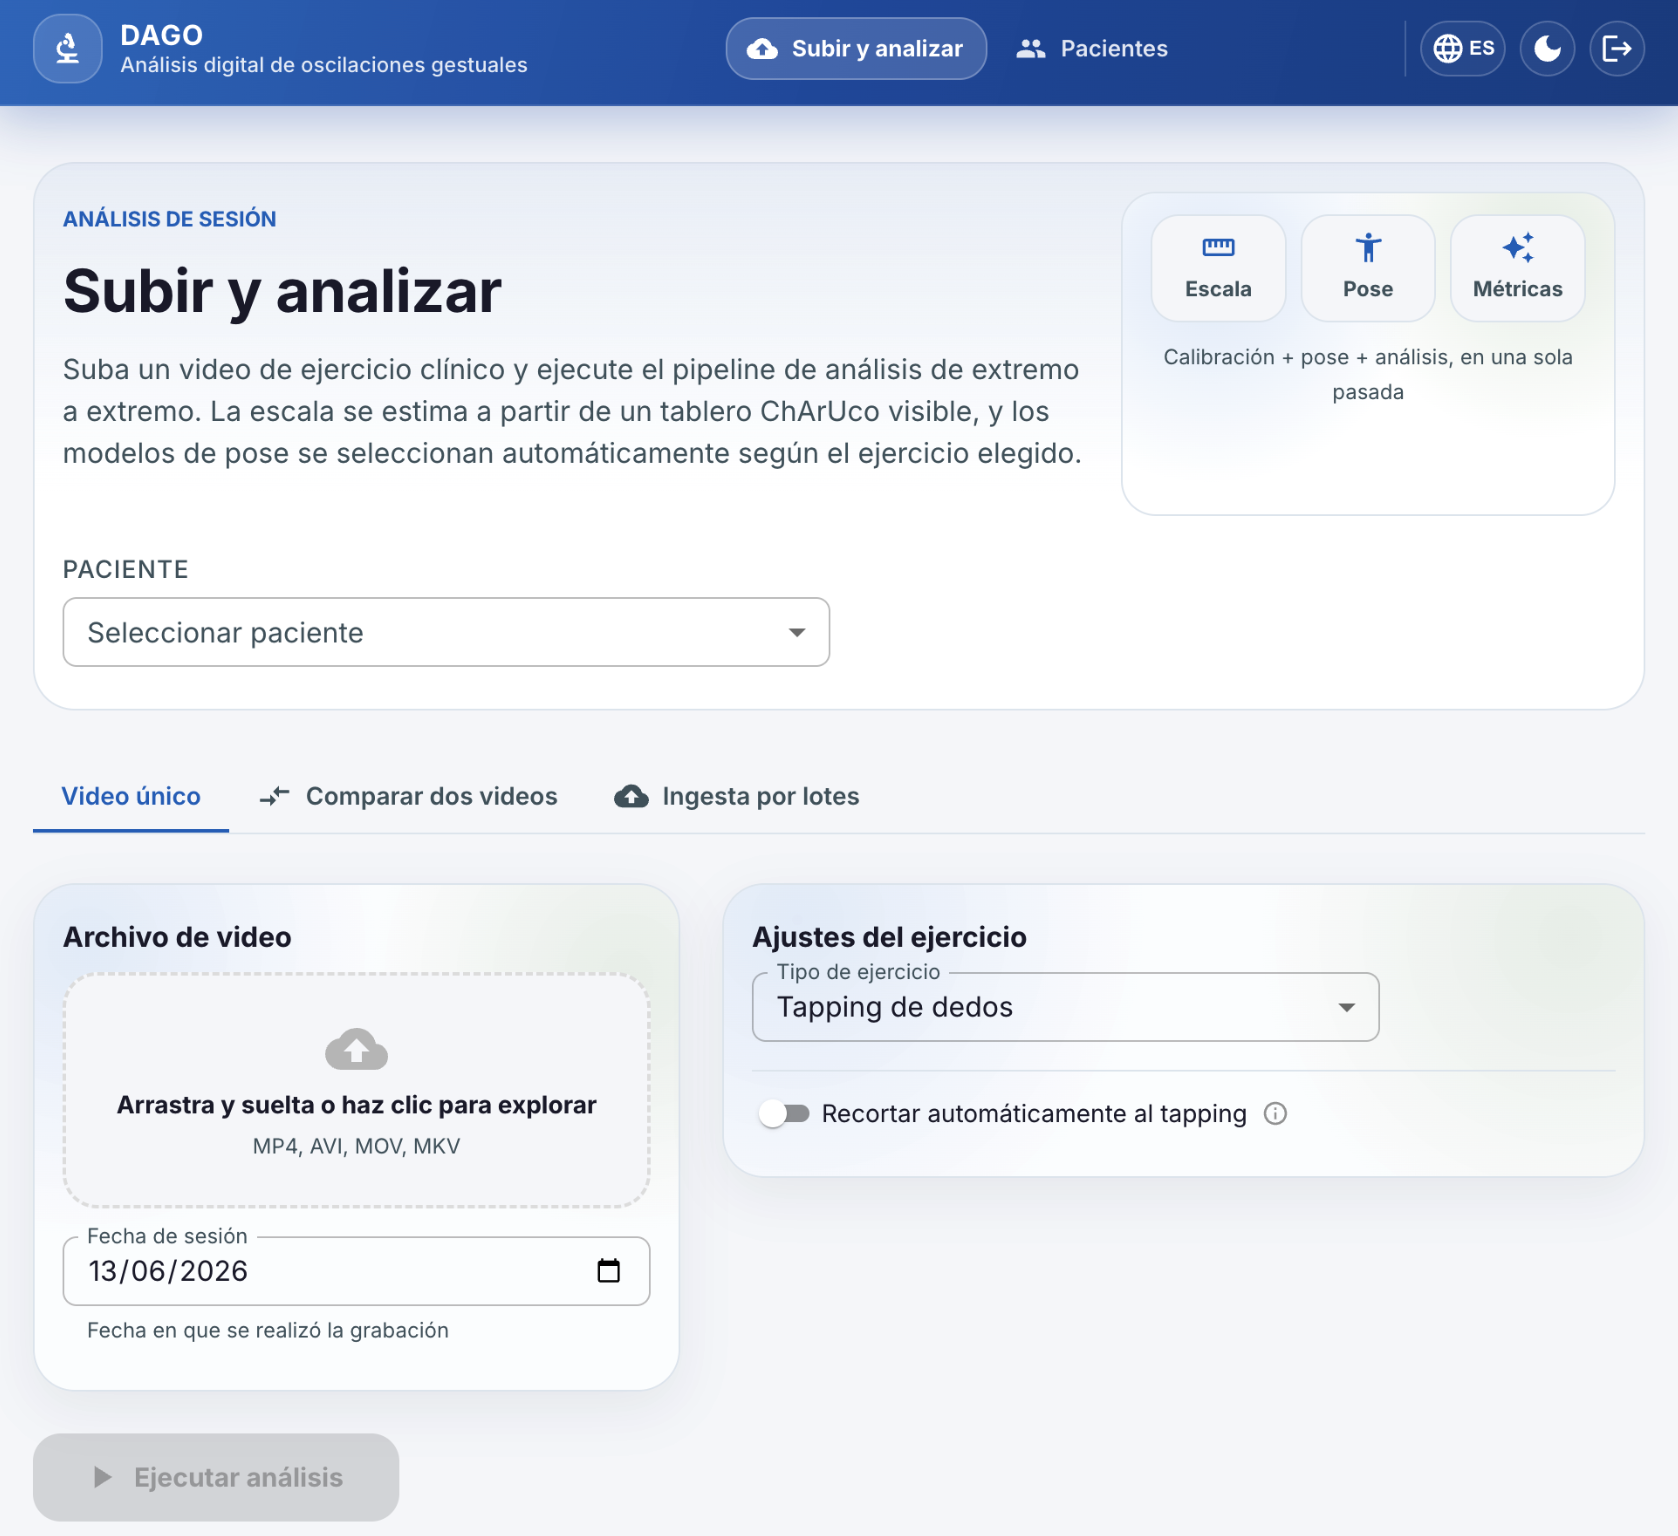
\includegraphics[width=0.80\textwidth]{Figures/cap_3/ui_1_pantalla_para_subir_videos.png}
\caption{Interfaz de carga de sesión.}
\label{fig:ui-upload}
\end{figure}

En la pantalla de resultados se combinan tablas de métricas con gráficos de series temporales construidos con una biblioteca de gráficos declarativos, superposición opcional de landmarks sobre el video y solicitud de resúmenes interpretativos bajo demanda.

La vista de detalle de paciente integra un componente de evolución que filtra sesiones previas por tipo de ejercicio y representa la tendencia de biomarcadores seleccionados a lo largo del tiempo, en apoyo del seguimiento longitudinal previsto en los objetivos del trabajo.

La página de comparación envía las métricas de dos sesiones al servicio de insights para obtener un texto contrastivo, sin transmitir imágenes ni identificadores del paciente al proveedor del modelo de lenguaje.

En la figura \ref{fig:ui-results} se presenta la vista de resultados de una sesión con gráficos de métricas, donde se omiten los datos identificables del paciente.

\vspace{0.6em}
\begin{center}
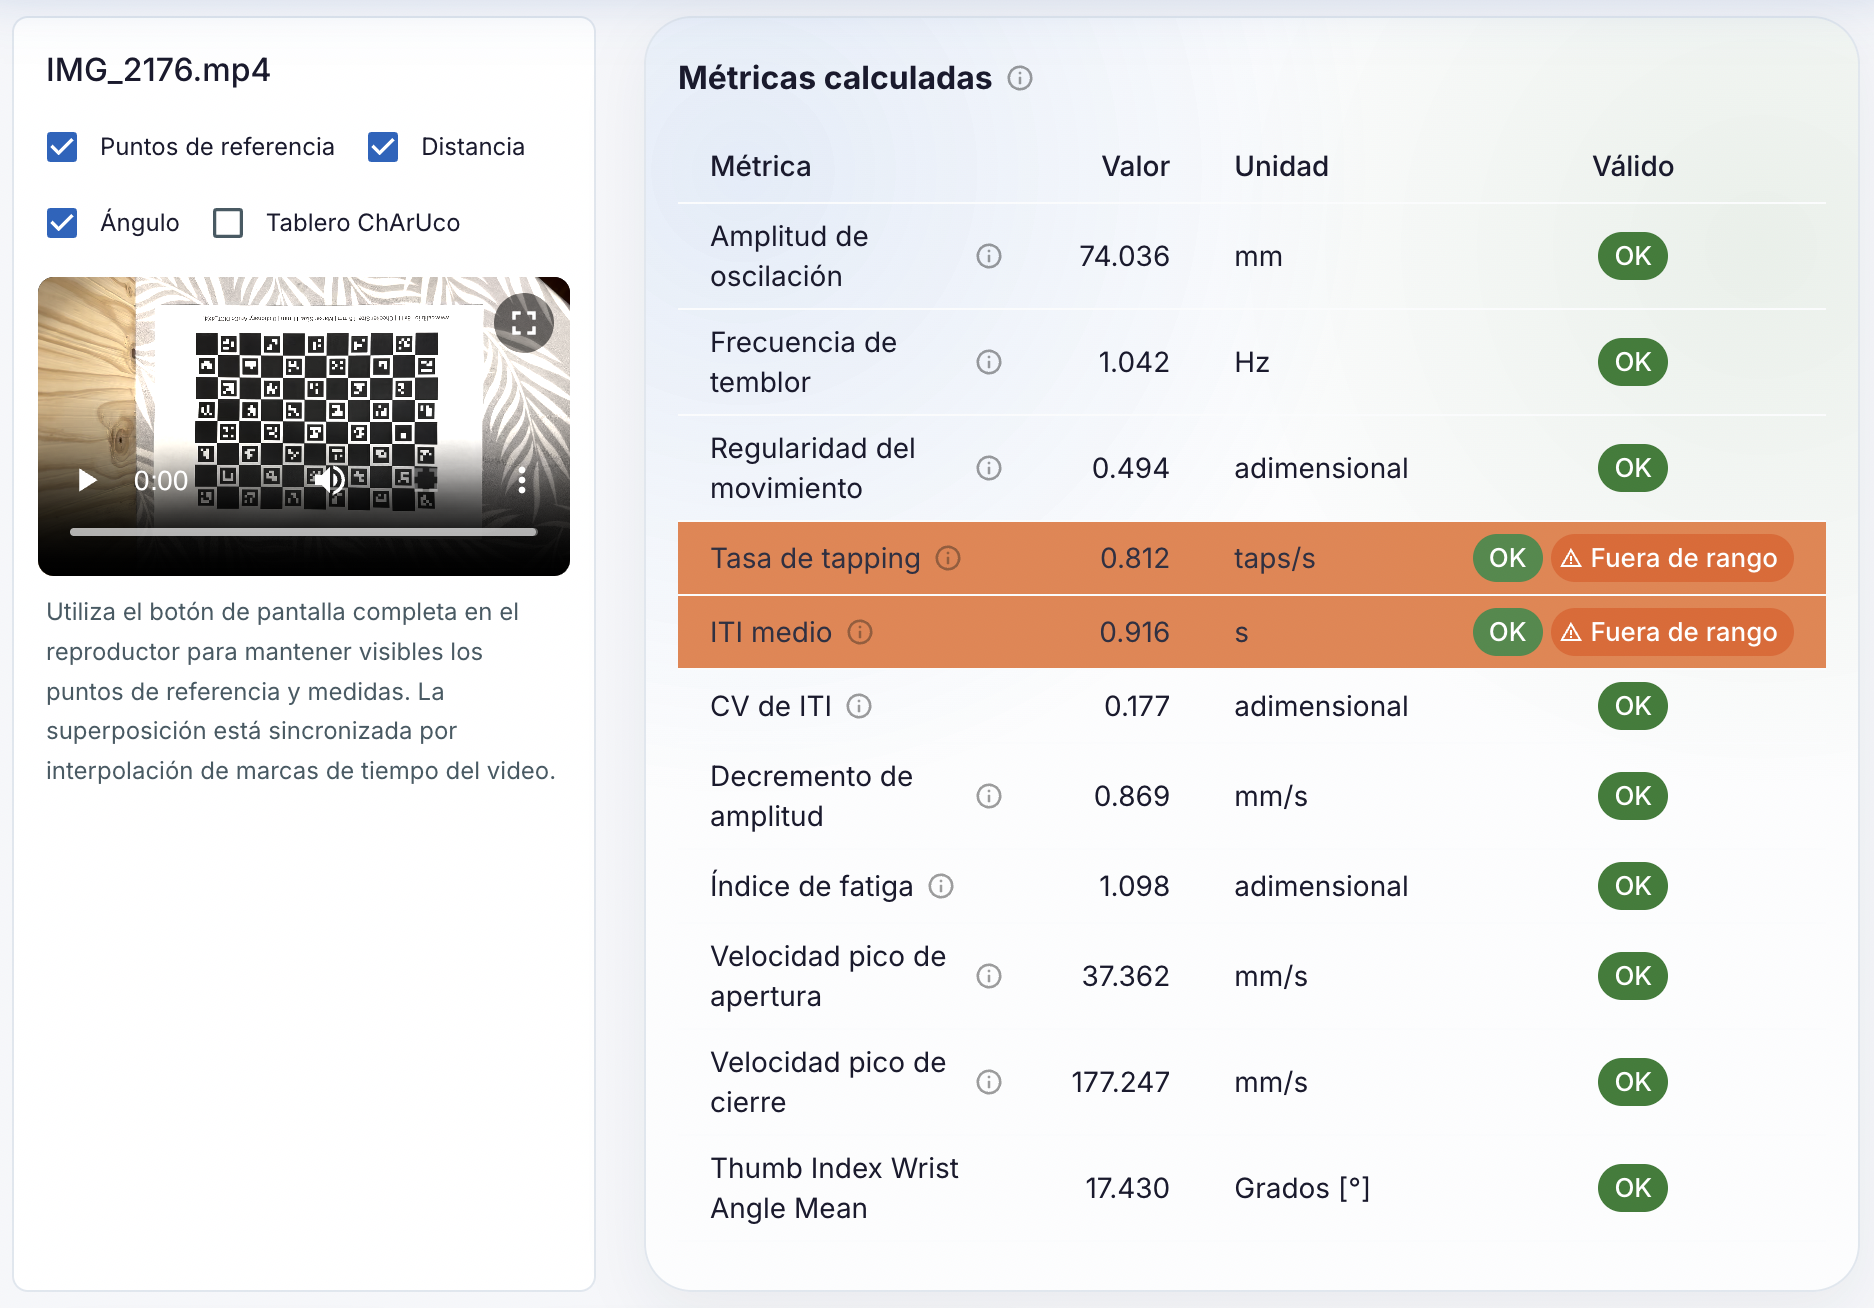
\includegraphics[width=0.85\textwidth]{Figures/cap_3/ui_2_resultados_sesion_2.png}
\captionof{figure}{Interfaz de visualización de resultados.}
\label{fig:ui-results}
\end{center}
\vspace{0.4em}

Los endpoints de interpretación envían al modelo de lenguaje únicamente métricas agregadas y metadatos no identificatorios, conforme a la política descrita en la sección \ref{sec:modelos-preentrenados}, y devuelven texto en lenguaje natural como apoyo a la lectura del informe.

\subsection{Despliegue local y en la nube}

\begin{sloppypar}
En entorno local, \texttt{Docker Compose} \citep{merkel2014docker} orquestó cuatro servicios principales: base de datos \texttt{PostgreSQL}~16, API en \texttt{Python}~3.12 (imagen multi-etapa con dependencias instaladas mediante \texttt{uv} y límite de memoria de 12~GiB), frontend con \texttt{nginx} en el puerto~3000 (build estático de \texttt{React} y proxy de la API en el puerto~8000) y el sidecar MeTRAbs descrito en la sección~\ref{sec:pipeline}. Este último se aisló en un contenedor propio de 10~GiB con interfaz \texttt{FastAPI} en el puerto interno~8081, de modo que la carga de \texttt{TensorFlow} no compitiera con \texttt{MediaPipe} en el servicio principal; la comunicación entre ambos contenedores se realizó por HTTP con autenticación por clave compartida.

Un perfil opcional permitió además ejecutar el mismo contenedor de la API en modo batch desde la línea de comandos. Los modelos de visión, los videos de muestra y el directorio de salida se montaron como volúmenes para facilitar la actualización sin reconstruir la imagen. La figura~\ref{fig:infra-local-dago} resume la topología local.
\end{sloppypar}

\begin{figure}[htbp]
\centering
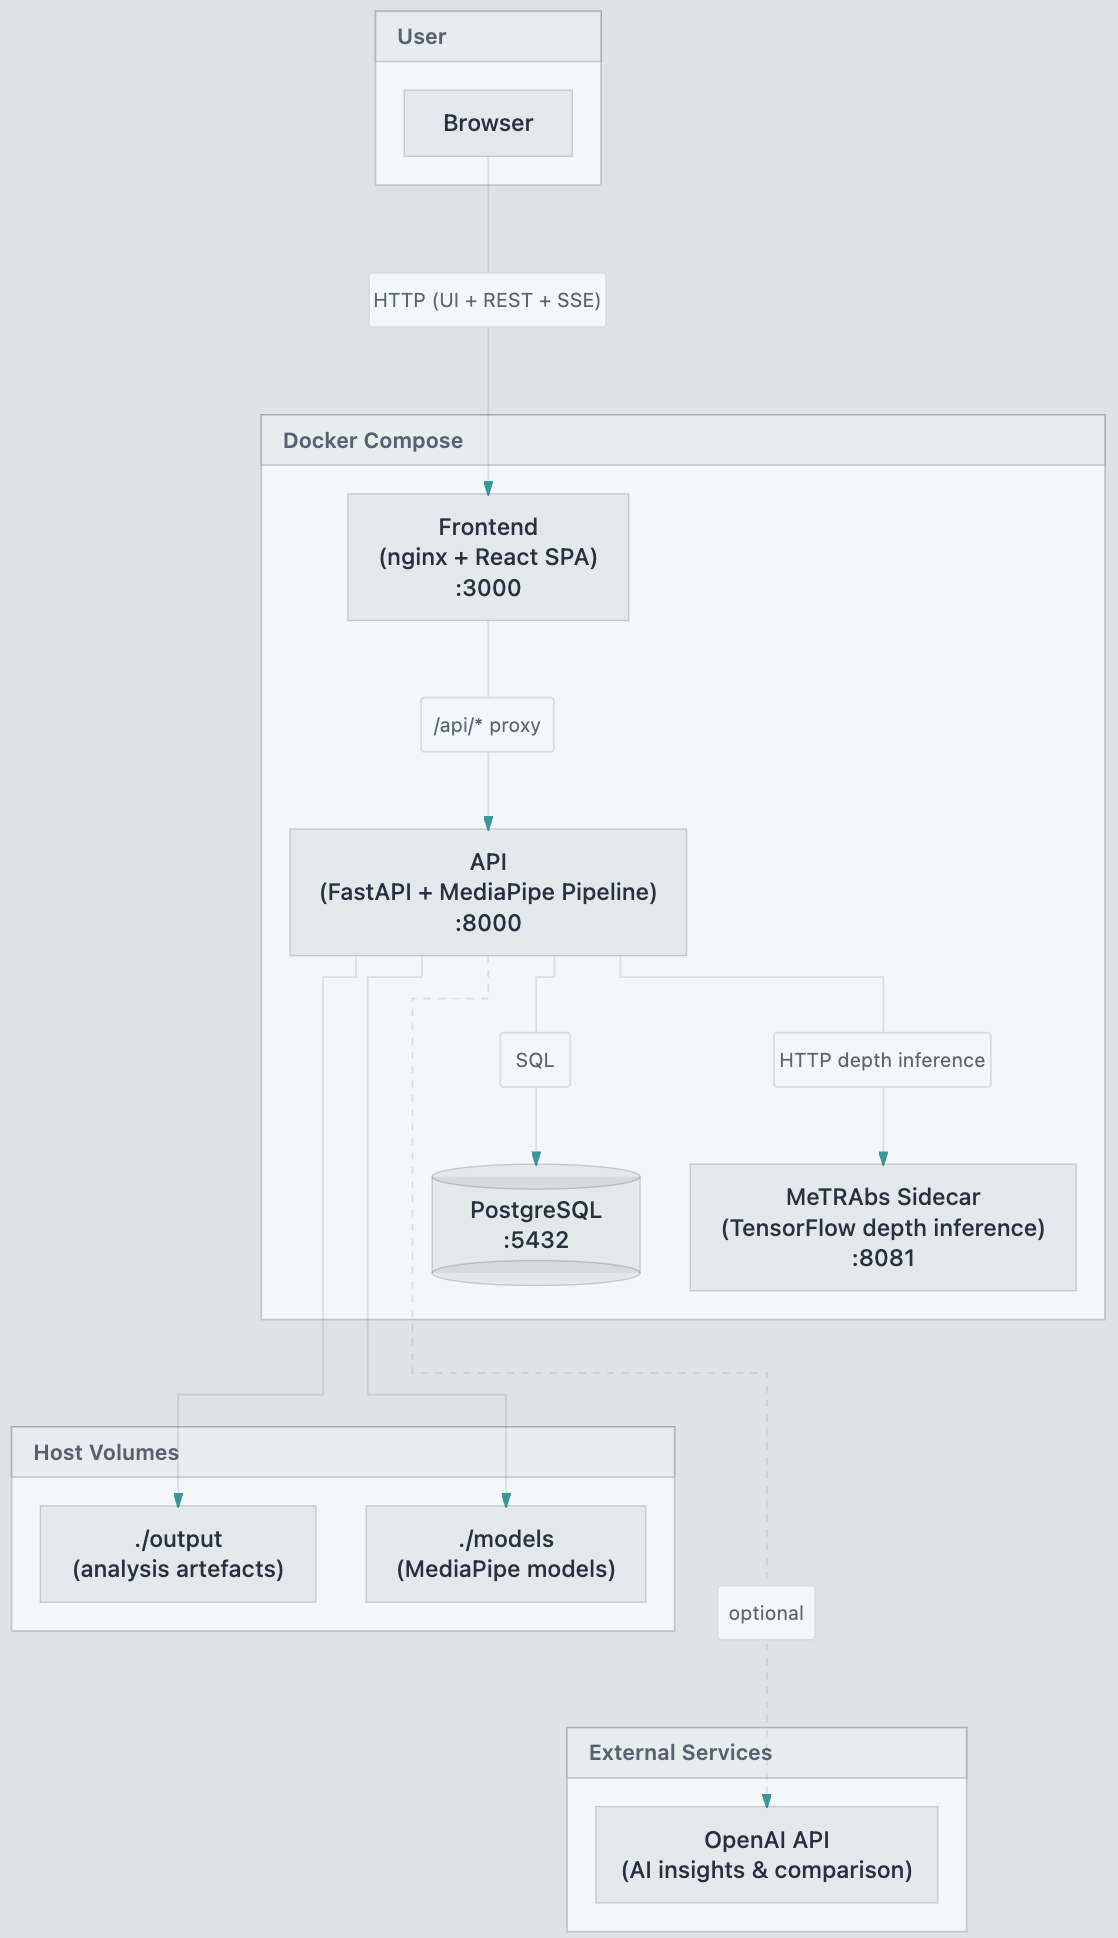
\includegraphics[width=0.88\textwidth]{Figures/cap_3/diagrama_bloques_infraestructura_dago_local.png}
\caption{Arquitectura de despliegue local con \texttt{Docker Compose}.}
\label{fig:infra-local-dago}
\end{figure}

\begin{sloppypar}
En el diagrama local se observa la separación entre el acceso web, el procesamiento analítico y la base de datos, con MeTRAbs como servicio independiente. El punto de entrada del contenedor de la API ejecutó migraciones de esquema con \texttt{Alembic} antes de levantar \texttt{uvicorn}, de modo que un despliegue nuevo aplicara automáticamente las revisiones pendientes. El frontend se construyó en una etapa previa de la imagen (\texttt{Node.js} para compilar TypeScript) y el runtime de inferencia se fijó en \texttt{linux/amd64} por compatibilidad con \texttt{MediaPipe}. La configuración del proxy desactivó el buffering en las rutas de la API y extendió el tiempo de lectura a 3600~s, requisito para transmitir el progreso del análisis mediante eventos enviados desde el servidor (SSE).
\end{sloppypar}

\begin{sloppypar}
Para la prueba de concepto en la nube se adaptó el diseño a los servicios gestionados de GCP enumerados en la tabla~\ref{tab:infra-gcp-cap2}, con el objetivo de reducir costos operativos y simplificar el despliegue inicial, sin replicar de forma idéntica la topología local. Un único servicio en \texttt{Cloud Run} concentró la API, el pipeline de análisis y la interfaz web empaquetada en el mismo contenedor; no se desplegó un proxy \texttt{nginx} separado ni el sidecar MeTRAbs. \texttt{Cloud SQL} alojó \texttt{PostgreSQL}~16 con conexión por socket Unix; \texttt{Cloud Storage} persistió videos y artefactos de sesión; \texttt{Secret Manager} inyectó las credenciales de base de datos y la clave de firma de tokens; \texttt{Cloud Build} construyó la imagen y la publicó en \texttt{Artifact Registry}.

Las migraciones de esquema se ejecutaron mediante un trabajo dedicado en \texttt{Cloud Run Jobs}, separado del arranque del servicio HTTP. La infraestructura se provisionó con \texttt{Terraform} en el entorno de prueba, con 4~vCPU, 8~GiB de memoria, concurrencia~1, tiempo máximo de 3600~s y CPU activa de forma continua para sostener hilos de procesamiento en segundo plano. La figura~\ref{fig:infra-gcp-dago} resume las relaciones entre el usuario, el cómputo serverless y los servicios de datos y secretos.
\end{sloppypar}

\begin{figure}[htbp]
\centering
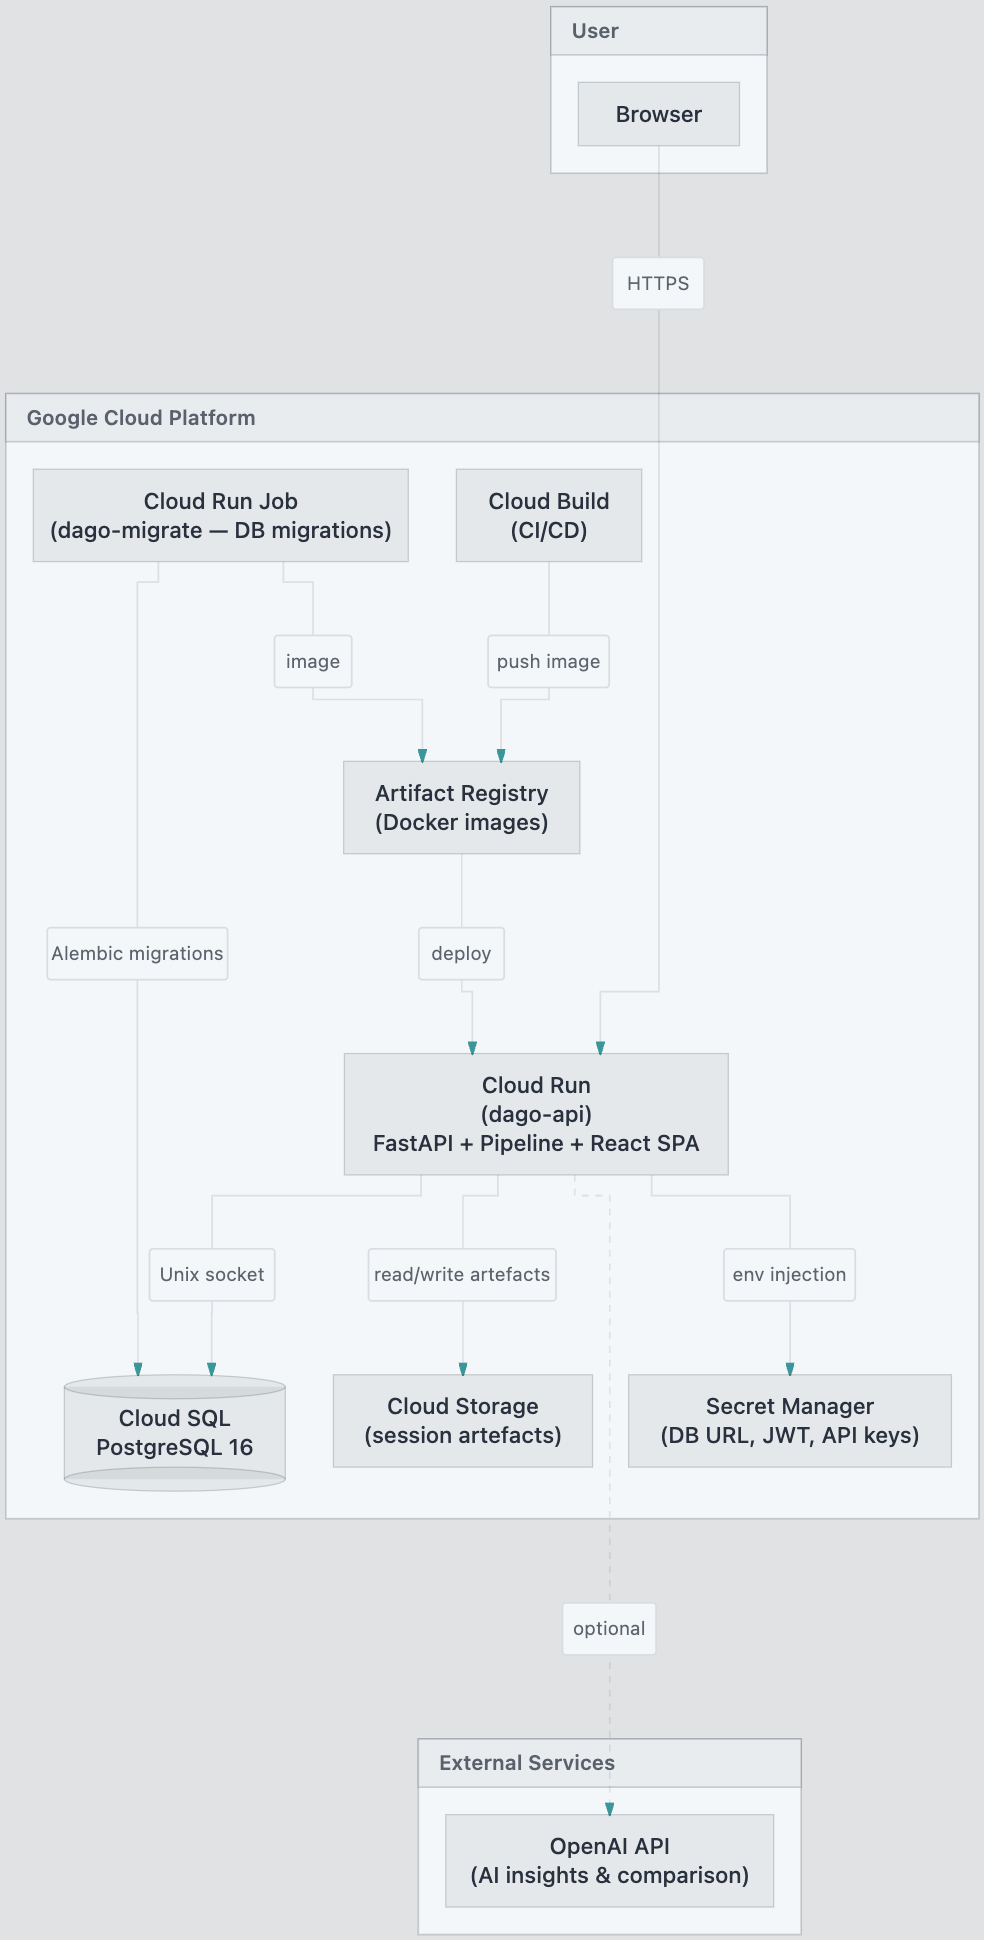
\includegraphics[width=0.88\textwidth]{Figures/cap_3/diagrama_bloques_infraestructura_dago_gcp.png}
\caption{Arquitectura de despliegue del prototipo en Google Cloud Platform.}
\label{fig:infra-gcp-dago}
\end{figure}

\begin{sloppypar}
En el diagrama de la nube se aprecia que el procesamiento de video y la inferencia con \texttt{MediaPipe} residen en el mismo servicio de cómputo que expone la API REST y sirve la interfaz web, mientras que la persistencia estructurada y los objetos de gran tamaño se externalizan a servicios administrados. Esa separación facilitó desplegar el prototipo sin duplicar el almacenamiento de videos en cada instancia, aunque el estado de progreso SSE permanece en memoria de proceso y el escalado horizontal quedó acotado a una sola réplica; ambas son limitaciones conocidas que se abordarán en el capítulo de conclusiones.
\end{sloppypar}
Con la arquitectura descrita quedó cerrado el ciclo de diseño e implementación: desde la captura estandarizada descrita en el capítulo anterior hasta la consulta web de métricas y exportación de informes. En el capítulo~\ref{Chapter4} se presentará el plan de evaluación y los resultados obtenidos al ejecutar este sistema sobre el conjunto de videos disponible para el trabajo, además de documentar la verificación automatizada del desarrollo, las pruebas unitarias y la integración de extremo a extremo del pipeline.


% Chapter Template

\chapter{Ensayos y resultados}

\label{Chapter4}

En este capítulo se presentó el plan de evaluación del sistema, las pruebas automatizadas que respaldaron la reproducibilidad del pipeline implementado en el capítulo~\ref{Chapter3} y los resultados obtenidos al ejecutar el prototipo sobre los videos disponibles para el trabajo.

%----------------------------------------------------------------------------------------
%	SECTION 1
%----------------------------------------------------------------------------------------

\section{Pruebas automatizadas del pipeline}
\label{sec:pruebas-automatizadas}

Durante el desarrollo se mantuvo una batería de pruebas unitarias sobre componentes aislados del flujo analítico: calibración ChArUco, detección de fase estática, impulsos de audio, métricas espectrales y de tapping, ángulos derivados y escritores de exportación. Los módulos bajo \texttt{tests/unit/} validaron comportamientos con señales sintéticas o entradas controladas, de modo que las definiciones matemáticas descritas en el capítulo~\ref{Chapter3} pudieran contrastarse con salidas esperadas. Se incluyó además una prueba de integración de humo (\texttt{tests/integration/test\_cli\_smoke.py}) que ejecutó el comando de sesión sobre un video de muestra del repositorio y verificó la generación de \texttt{tracking.csv}, \texttt{metrics.csv} y \texttt{summary.json} con esquemas estables.

Esas pruebas no sustituyeron la validación clínica formal, excluida del alcance del trabajo, pero demostraron que el ensamblado descrito en el capítulo de diseño era reproducible y detectaba regresiones en el flujo de extremo a extremo.

%----------------------------------------------------------------------------------------
%	SECTION 2 — plan de evaluación, resultados y análisis (por completar)
%----------------------------------------------------------------------------------------

% Chapter 5

\chapter{Conclusiones}

\label{Chapter5}

En este capítulo se presentan las conclusiones del trabajo. Se analiza el grado de cumplimiento de los objetivos enunciados en el capítulo~\ref{Chapter1}, se repasan los conocimientos de la carrera aplicados durante el desarrollo y se proponen líneas de continuidad para el sistema.

%----------------------------------------------------------------------------------------
%	SECTION 1
%----------------------------------------------------------------------------------------

\section{Logros alcanzados}

El objetivo general del trabajo se cumplió: se diseñó e implementó un sistema de análisis digital de oscilaciones y desempeño motor que procesa videos de ejercicios clínicos asociados a la enfermedad de Parkinson, deriva métricas cuantitativas mediante estimación automática de pose y procesamiento de señales, y las presenta en visualizaciones orientadas al personal de salud.

Los objetivos específicos del capítulo~\ref{Chapter1} quedaron cubiertos en lo esencial. Se construyó un flujo completo desde la ingesta de video hasta la exportación de resultados, con calibración espacial, seguimiento temporal y cálculo de métricas diferenciadas según el tipo de ejercicio clínico. Se integraron modelos preentrenados de estimación de pose y se desarrolló la capa de exposición mediante servicios web, interfaz gráfica, informes exportables y vistas de seguimiento longitudinal. La efectividad de la implementación se verificó mediante pruebas automatizadas y ensayos de integración en entornos local y en la nube, con resultados favorables en su conjunto y deuda técnica acotada, según el análisis del capítulo~\ref{Chapter4}.

El sistema superó el alcance mínimo inicial al incorporar comparación entre sesiones, interpretación asistida sobre métricas agregadas y despliegue reproducible en contenedores y en una prueba de concepto en infraestructura gestionada \citep{gcp,merkel2014docker}. La retroalimentación de profesionales de la salud, entre neurólogos y kinesiólogos, fue positiva respecto de la utilidad de las métricas y de los informes, y orientó mejoras en la presentación de resultados y en el seguimiento entre sesiones.

El cumplimiento no fue absoluto en todos los frentes planificados. Las salvaguardas de privacidad, el portal de paciente y la cobertura plena de las pruebas de integración con material de video real quedaron en estado parcial o condicionado. Esas brechas se abordan en la sección~\ref{sec:trabajo-futuro}.

Frente al estado del arte, el trabajo se inscribió en la línea de plataformas de análisis markerless basadas en visión por computadora, como las revisadas en el capítulo~\ref{Chapter1} \citep{acevedo2025visionmd,sibley2021video,pecoraro2025computer}. El aporte diferencial radica en la orientación a servicios, la portabilidad entre entornos de ejecución y el seguimiento longitudinal multiejercicio en una misma herramienta. No corresponde afirmar superioridad diagnóstica: la evaluación verificó la implementación y no la concordancia con escalas clínicas de referencia, de modo que el sistema debe entenderse como complemento objetivo de la evaluación habitual y no como su reemplazo.

%----------------------------------------------------------------------------------------
%	SECTION 2
%----------------------------------------------------------------------------------------

\section{Conocimientos aplicados}

El desarrollo articuló conocimientos de distintas áreas de la carrera. Del aprendizaje automático y la visión por computadora se aplicaron criterios para seleccionar, integrar y orquestar modelos preentrenados, con atención a sus condiciones de validez, su costo computacional y sus limitaciones ante condiciones adversas de captura. La capa interpretativa basada en un modelo de lenguaje exigió además nociones de diseño de instrucciones, control de la generación y resguardo de datos sensibles.

Del procesamiento de señales y la estadística se emplearon técnicas de análisis temporal y espectral, detección de eventos en series cinemáticas, medidas de variabilidad y regularidad, y agregación por sesión para apoyar la lectura clínica de los resultados.

De la ingeniería de software se aplicaron diseño modular, contratos de datos entre etapas, pruebas automatizadas, persistencia relacional, desarrollo de servicios y aplicaciones web, empaquetado con contenedores e infraestructura como código. También se consideraron prácticas de manejo responsable de datos de salud acordes a los requerimientos éticos de la planificación inicial.

%----------------------------------------------------------------------------------------
%	SECTION 3
%----------------------------------------------------------------------------------------

\section{Trabajo futuro}
\label{sec:trabajo-futuro}

Las líneas de continuidad se agrupan en datos, arquitectura, despliegue y validación clínica.

En materia de datos, la prioridad es conformar un conjunto de grabaciones más amplio y anotado, bajo consentimiento informado y resguardo regulatorio, que habilite estudios de concordancia entre las métricas del sistema y puntuaciones clínicas de referencia \citep{sibley2021video}. También conviene completar la cobertura de pruebas de integración en el entorno de desarrollo continuo.

En la arquitectura del sistema quedan mejoras identificadas durante los ensayos: cerrar la deuda técnica residual en las pruebas automatizadas, externalizar el estado de progreso de los análisis para habilitar escalado horizontal, medir de forma sistemática el rendimiento por sesión y explorar el uso de información de profundidad para un análisis tridimensional del movimiento \citep{guarin2025postural}.

En el plano del despliegue y el cumplimiento normativo, el paso hacia un uso clínico productivo exige endurecer las salvaguardas de privacidad hasta alcanzar conformidad plena con marcos regulatorios aplicables \citep{hipaa1996}. Finalmente, la validación clínica prospectiva con evaluadores independientes y protocolos de captura estandarizados constituye el paso necesario para transformar el prototipo verificado en una herramienta de apoyo a la decisión con evidencia de validez diagnóstica \citep{pecoraro2025computer}.


%----------------------------------------------------------------------------------------
% Apéndices
%----------------------------------------------------------------------------------------

\appendix

% Incluir apéndices desde archivos separados si es necesario
%\include{Appendices/AppendixA}

%----------------------------------------------------------------------------------------
% Bibliografía
%----------------------------------------------------------------------------------------

\renewcommand{\bibname}{Bibliografía} % Para asegurarte de que el título sea correcto
\phantomsection % Necesario para que el enlace del marcador sea correcto

\printbibliography[heading=bibintoc]

\end{document}






